%% 美赛模板:正文部分

\documentclass[12pt]{article}  % 官方要求字号不小于 12 号,此处选择 12 号字体

% 本模板不需要填写年份,以当前电脑时间自动生成
% 请在以下的方括号中填写队伍控制号
\usepackage[2506135]{easymcm}  % 载入 EasyMCM 模板文件
\problem{C}  % 请在此处填写题号
\usepackage{mathptmx}  % 这是 Times 字体,中规中矩 
%\usepackage{mathpazo}  % 这是 COMAP 官方杂志采用的更好看的 Palatino 字体,可替代以上的 mathptmx 宏包
\usepackage{amsmath}
\usepackage{tabularray}
%拉取的一些宏包
\usepackage{graphicx} 
%\usepackage{pdfpages}
\usepackage{longtable}
%\usepackage{tabu}
\usepackage{threeparttable} %支持在表格中使用 \tnote 命令添加脚注,并自动编号
\usepackage{listings} %在文档中插入代码
%\usepackage{paralist}%创建紧凑的列表,节省垂直空间
%\usepackage{setspace} %调整文档的行间距
%\usepackage{booktabs}%用于创建更美观的表格,提供了高质量的表格线条命令,如 \toprule、\midrule 和 \bottomrule
%\usepackage{makecell} %创建多行单元格,支持复杂的表格布局
\usepackage{amssymb} %提供了额外的数学符号,通常与 amsmath 宏包一起使用
\usepackage{appendix} %管理附录部分,自动处理附录的编号和格式
\newcommand{\upcite}[1]{\textsuperscript{\textsuperscript{\cite{#1}}}}


\title{Together, Individuals Make a Difference}  % 标题

% 如需要修改题头(默认为 MCM/ICM),请使用以下命令(此处修改为 MCM)
%\renewcommand{\contest}{MCM}

% 文档开始
\newtheorem{keywords}{Keywords}
\begin{document}

% 此处填写摘要内容
\begin{abstract}
The Olympic Games serve as both a stage for athletes' performances and a focal point for global competition in the medal table. This study aims to predict the medal distribution for the 2028 Olympics using a bottom-up approach, estimating the total medal count for each country based on individual athletes' expected performance. To achieve this, multiple predictive models were developed to forecast the future medal table and uncover deeper data features, providing valuable decision-making insights for national Olympic committees.

In Task 1, data preprocessing and feature engineering were first performed, utilizing KMeans++ and other statistical methods to extract latent features. Subsequently, the LightGBM model was employed to predict the number of gold, silver, and bronze medals for each country at the 2028 Olympics. 
The results indicate that a country's medal performance is closely related to factors such as home advantage, adeptness in specific events, and the individual performance levels of athletes. The model demonstrated high accuracy, with an R² value of 0.890 for the gold medal prediction, suggesting the reliability of the results.

For countries yet to win medals, our research revealed that participation in high-growth potential events increases the likelihood of securing their first medal. Spearman Correlation Analysis further examined the degree of dependency on specific events by certain countries. The findings show that countries with strong overall sports performance exhibit a lower dependency on specific events, maintaining stable results, while weaker sports nations tend to rely more on select events. In some cases, the correlation coefficient in athletics events was as high as 0.894, indicating a concentration of athletic development in a few specific areas.

In Task 2, we explored the "great coach effect" by applying Bayesian Change Point Detection (BEAST) to analyze instances from multiple countries. The study found a significant correlation between the points of inflection in some countries' sports performance and the tenure of a "great coach," validating the importance of this effect.

Additionally, forward CUSUM analysis was employed to examine changes in medal sequences, identifying the weakest areas for each country. The results show that many countries, which once had competitive advantages in certain events, have seen a decline in these advantages over time. Based on this, we propose targeted coach recommendations for countries in need of improvement in specific areas.

In Task 3, we conducted in-depth data mining and analysis based on the models and data mentioned earlier, revealing several novel insights, such as the gender ratio of athletes, advantages derived from a country's traditional events, and changes in medal counts reflecting shifts in international political dynamics.

The study found that the gender ratio in the Olympics is gradually balancing, with a significant increase in the proportion of female medals.

Furthermore, some countries dominate traditional events, with their medal share reaching up to 88. Consequently, Olympic committees seeking to increase their medal counts should consider investing more in their national traditional events. 

Finally, through time-series analysis of changes in medal distribution, multiple anomalies were identified, reflecting not only the evolution of the Olympics from its early stages to maturity but also their connection to the political context of the 20th century.


    % 美赛论文中无需注明关键字。若您一定要使用,
    % 请将以下两行的注释号 '%' 去除,以使其生效
    % \vspace{5pt}
    % \textbf{Keywords}: MATLAB, mathematics, LaTeX.
    
    
 
 
    % 关键字Keywords
    \vspace{5pt}
    \textbf{Keywords}: \textbf{ A, B, C,  }
    
	
\end{abstract}

\maketitle  % 生成 Summary Sheet
\tableofcontents  % 生成目录


% 正文开始
\section{Introduction}
\subsection{Problem Background}
During the 2024 Paris Summer Olympics, fans not only paid attention to the individual events but also showed significant interest in the the ranking of countries on the medal table. Ultimately, the United States topped the medal table with a total of 126 medals, while China and the United States are tied for first place in the number of gold medals, each securing 40 golds. The host country, France ranks 5th in the total number of gold medals with 16 gold medals, but finished 4th in the total medal count. Great Britain ranked 7th on the gold medal table with 14 golds, while securing 3rd place in the overall medal count. Despite the prominence of the leading countries, the medal achievements of other nations also attracted attention. For example, Albania, Cape Verde, Dominica, and Saint Lucia each won their first-ever Olympic medal in this edition of the Games, with Dominica and Saint Lucia each earning another gold medal. However, over 60 countries have yet to win a medal in the history of the Olympics. 
\subsection{Restatement of Problem}
While predictions of the final medal counts at the Olympics are common, such forecasts are generally not based on historical medal tables. Instead, they are typically made before the start of the upcoming Olympic Games, once the list of competing athletes is known.To clarify the task, the problem is restated as follows:

\begin{itemize}
	\setlength{\parsep}{0ex} %段落间距
	\setlength{\topsep}{2ex} %列表到上下文的垂直距离
	\setlength{\itemsep}{1ex} %条目间距
	\item Develop a model for each country’s medal count, which should at least include the number of gold medals and the total medal count, and estimate the uncertainty/precision of the model,also evaluate its performance.
		\begin{itemize}
		\item[1)]
Using the model, predict the medal standings for the 2028 Los Angeles Summer Olympics, including prediction intervals for all outcomes. Based on the model’s predictions, identify which countries are most likely to improve their performance and which countries are expected to perform worse than in the 2024.
	\end{itemize}
	\begin{itemize}
		\item[2)]
		The developed model should include countries that have not yet won any medals, while also predicting the number of countries likely to win their first medal in the upcoming Olympics and provide odds for this estimate.
	\end{itemize}
		\begin{itemize}
		\item[3)]
The model should also consider the number and types of events in each specific Olympic Games, exploring the relationship between the events and the number of medals won by each country. For each country, determine which events are most crucial and why, as well as the impact of the country’s selected events on the results.
	\end{itemize}
	
	
	\item In contrast to athletes, who must change their citizenship in order to represent different countries in competitions, coaches do not need to change their citizenship to coach, which makes it easier for them to move to other countries. As a result, the “great coach” effect may arise. For example, Lang Ping has coached the volleyball teams of both China and the U.S., leading both to championships, while Bela Karolyi coached the Romanian and U.S. women’s gymnastics teams, achieving great success. The task is to identify evidence in the data that may suggest changes driven by the "great coach" effect and estimate its impact on the medal count. Select 3 countries, determine the events in which they should consider investing in "great" coaches, and estimate the potential impact of such investments.
	\item Explain the unique insights regarding Olympic medal counts that are included in the developed model and how these insights can provide valuable information to the National Olympic Committees of various countries.

\end{itemize}

\subsection{Our work}
We do such things ...




%图片示例(water.png)
%\begin{figure}[htbp]
%	\centering
%	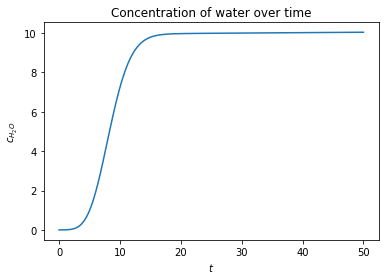
\includegraphics[width=.8\textwidth]{water.png}
%	\caption{The result of Model 2}\label{fig:result}
%\end{figure}
\begin{enumerate}[\bfseries 1.]
    \item We do ...
    \item We do ...
    \item We do ...
\end{enumerate}
\section{Question Preparation}
\subsection{Assumptions}
\textbf{Assumption 1 } \textit{The number of medals won by each country typically fluctuates only slightly from year to year, without significant increases or decreases.}

The total medal count of a country more accurately reflects the long-term investments and developmental outcomes in sports, rather than short-term results that can be drastically altered. Furthermore, external factors that influence medal counts, such as the organization of international competitions, rule changes, and judging standards, tend to remain relatively stable in the short term.


\textbf{Assumption 2 } \textit{Each year, a number of new athletes join the Olympic Games, some of whom may be competing for the first time. The specific proportion of these athletes will be estimated through our simulation. }

The performance variability of athletes is assumed to be limited, with minimal occurrences of exceptional overperformance or underperformance.  


\textbf{Assumption 3} \textit{ The performance variability of athletes is assumed to be limited, with minimal occurrences of exceptional overperformance or underperformance.  }

The performance variability of athletes is assumed to be limited, with minimal occurrences of exceptional overperformance or underperformance.  
Due to the systematic nature of athlete training and the relative consistency of competition environments, their performance tends to remain stable. By mitigating the impact of outliers, the model can avoid being influenced by extreme values.  

\subsection{Notations}

The primary notations used in this paper are listed in Table \ref{tb:notation}.

% 三线表示例
\begin{table}[!htbp]
\begin{center}
\caption{Notations}
\begin{tabular}{cl}
	\toprule
	\multicolumn{1}{m{3cm}}{\centering Symbol}
	&\multicolumn{1}{m{8cm}}{\centering Definition}\\
	\midrule
	$C_{i}$&Certain country\\
	$E_{i}$&Specific event\\
	$G$&Gold medal count\\
	$V$&Silver medal count\\
	$B$&Bronze medal count\\
	$M$&Total count of the 3 types of medals\\
	$A$&Number of new athletes\\
	$T$&Times of Olympic participations\\
    $\gamma$&Sport Advantage Coefficient\\
  	$ m_{c_{i}}$ &Total medal count of a certain country\\
	$ m_{c_{i},e_{j}}$ &Total medal count of a certain country in a specific event\\
	$L_{i}$&Country clustering level\\
    $g_{i}$&the second one\\
    $X$&Historical total medal counts (gold, silver, and bronze) of all countries\\
    $\xi$&The Probability of First Medal\\
    $\sigma$&                        \\
    $   $&Normalized version of probability of first medal         \\
	\bottomrule
\end{tabular}\label{tb:notation}
\end{center}
\end{table}

\section{Data Preprocessing}
\subsection{Basic Data Preprocessing}
Due to various influencing factors, there are significant differences in the competitive levels of countries in the Olympic Games, which have been reflected in past competitions, specifically in the total number of gold, silver, and bronze medals won by each country. 

To illustrate the differences in the levels of countries in previous Olympic Games (i.e. national level), we employed the KMeans++ clustering algorithm. Based on the number of gold, silver, and bronze medals, as well as the total medal count of each country in past Olympics, we classified the countries into five levels. These five levels, L1, L2, L3, L4, and L5, form a partition of the sample set X (the total number of gold, silver, and bronze medals won by countries in previous Olympic Games).
\begin{equation}
G_{i} \cap G_{j}=\emptyset, \bigcup_{i=1}^{5} G_{i}=X
\end{equation}
After the classification, the distribution of countries across the 5 levels is shown in the figures:
\begin{figure}[htbp]
	\centering
	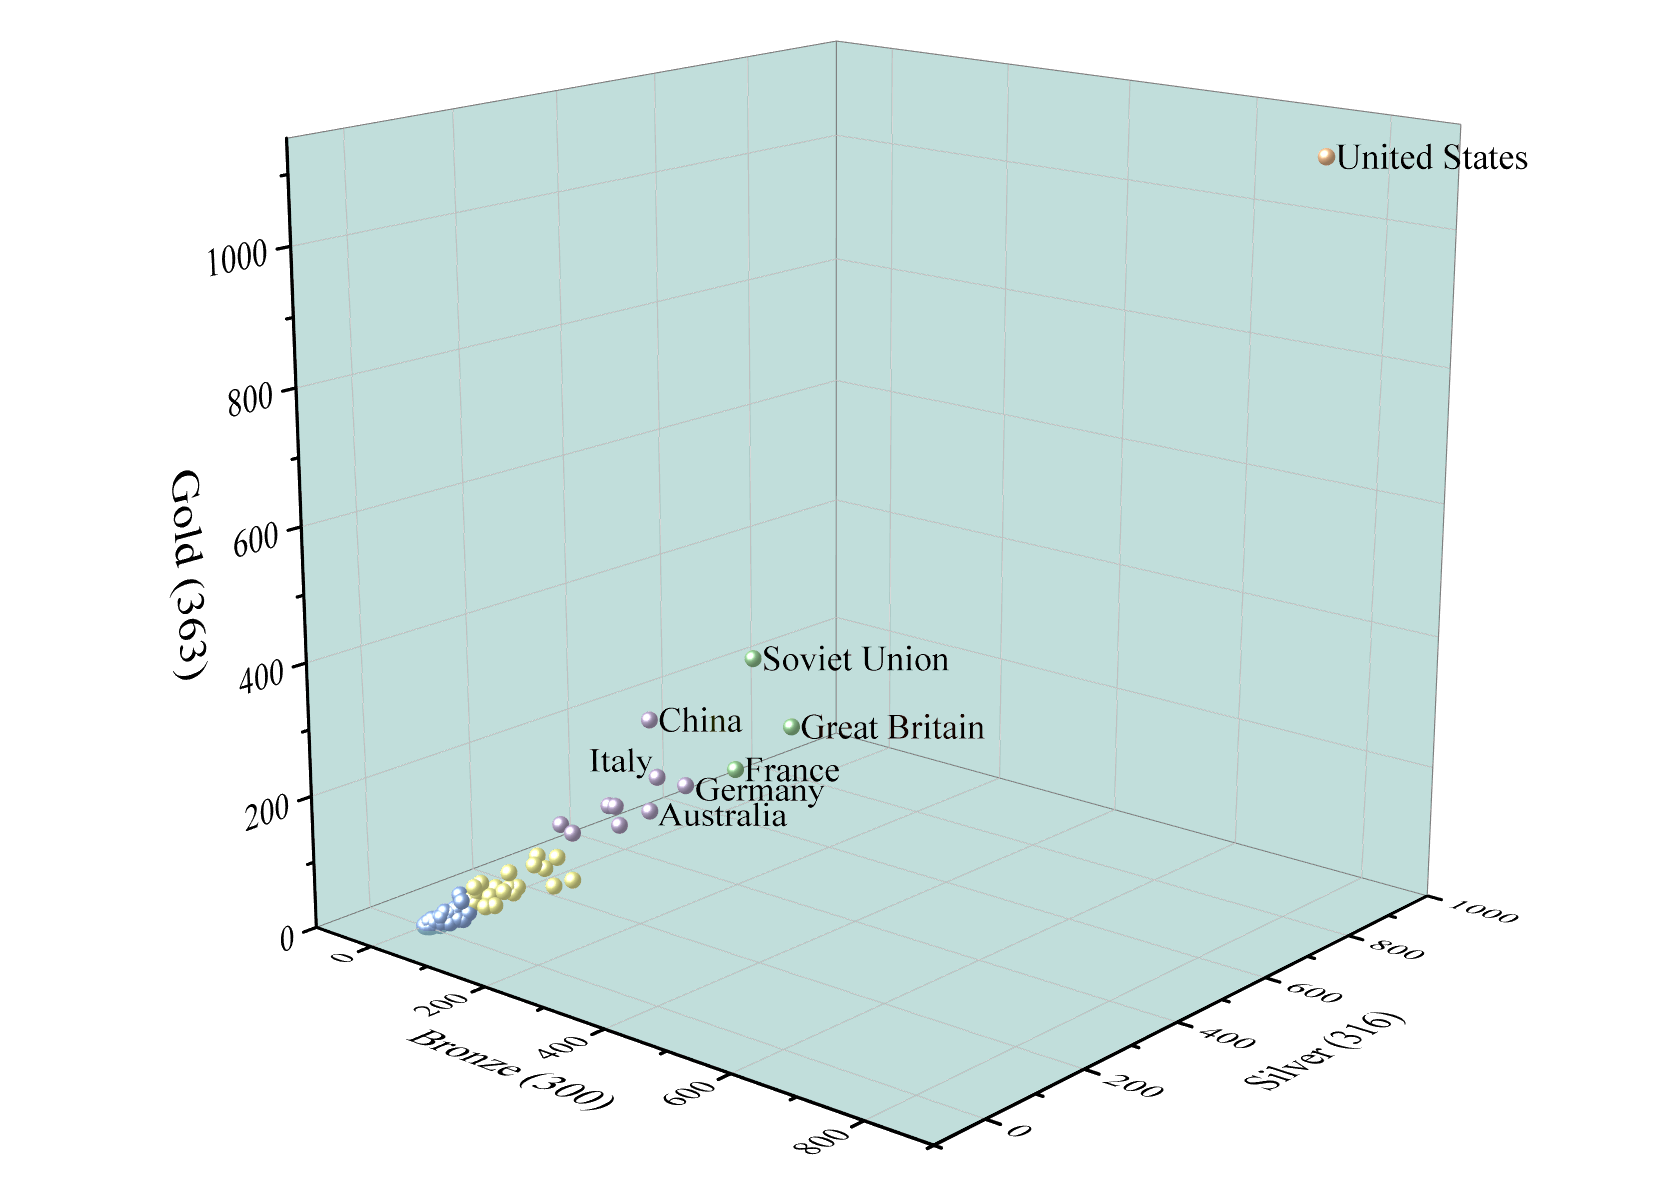
\includegraphics[width=12cm]{img/Level1.png}
	\caption{Scatter plot of national level classification (based on Kmeans++clustering algorithm)}
	\label{fig:aa}
\end{figure}

\begin{figure}[htbp]
	\centering
	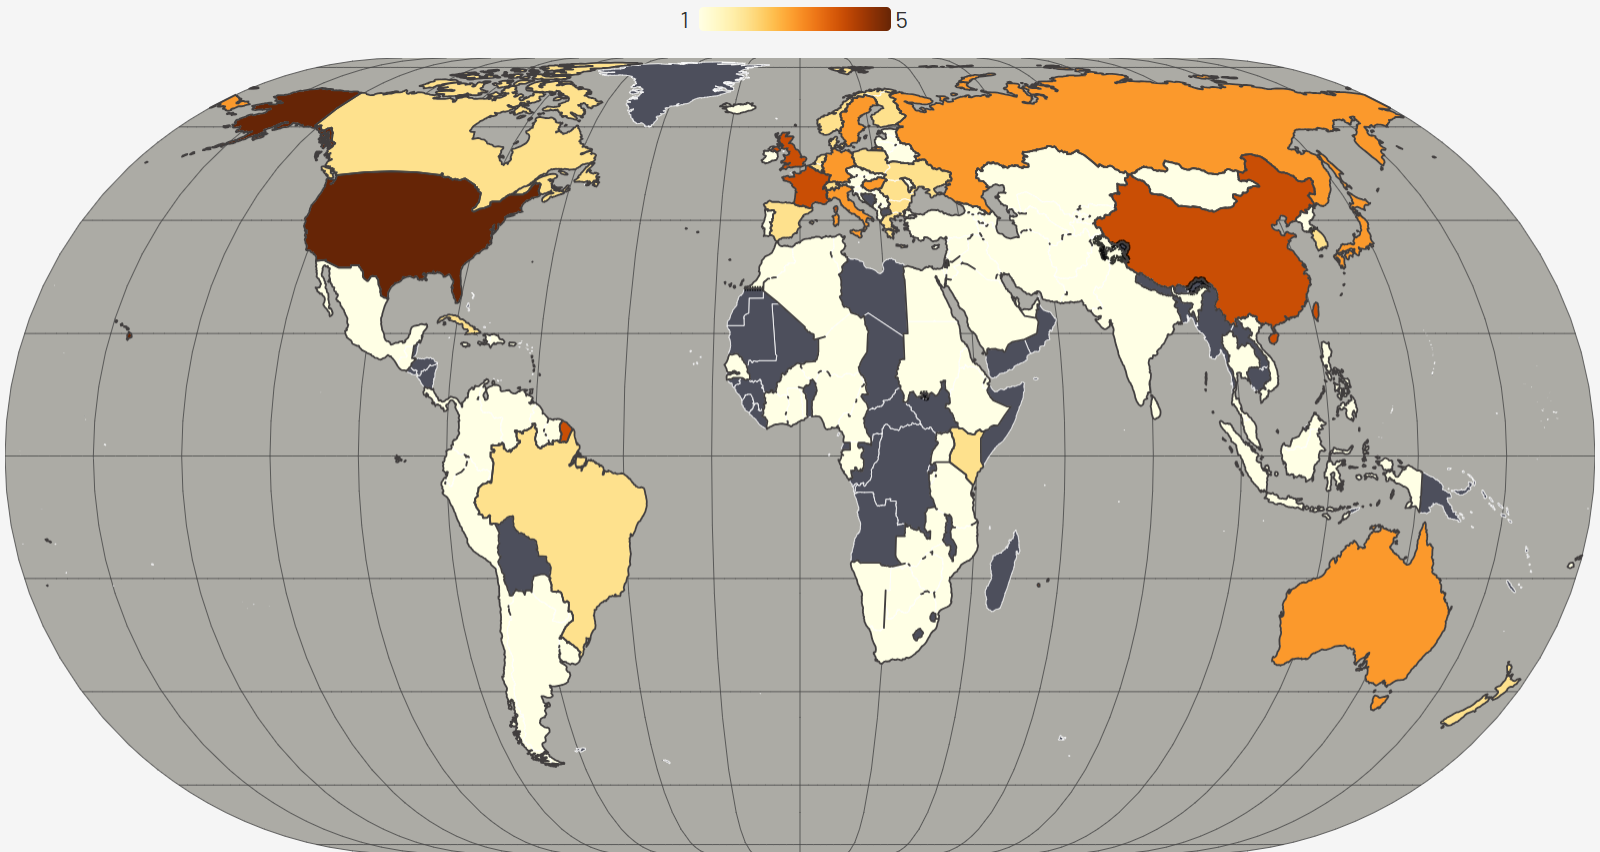
\includegraphics[width=12cm]{img/Level2.png}
	\caption{Geographical Distribution Map of Country Level Classification}
	\label{fig:aa}
\end{figure}


In addition, we created 10 new features based on the original variables, which were utilized during the modeling process with the LightGBM model.

%Table 2 :变量名表 Variable Name
\begin{longtblr}[
	caption = {Variable Name},
	]{
		vline{1-4} = {1-10}{},
		hline{1-11} = {1-3}{},
	}
	Variable Name                                                    & \textit{Code}                                                & Definition                                                                      &  \\
	Whether~Host Country                                             & \textit{is host}                                             & {Whether the country is the host(1 for host,0 for\\~non-host)}                  &  \\
	{Medal Expectation\\Increment *Personnel\\Expectation lncrement} & {\textit{medal\_increment *}\\\textit{personnel\_increment}} & {Product of medal\\expectation increment and\\personnel expectation\\increment} &  \\
	{Sport Advantage\\Coefficient}                                 & \textit{sport\_adv}                                           & {Advantage coefficient of\\a specific sport}                                  &  \\
	Country Level                                                    & \textit{country\_lvl}                                        & {The level of the country in the competition\\(ordered by rank)}                &  \\
	{Project Medal\\Expectation /Project\\Personnel Expection~}                         & \textit{sport\_medal \_per\_ person}                          & {Ratio of sport medals to projected personnel\\for a specific sport}          &  \\
	Gold Medal Probability                                           & \textit{gold\_prob}                                          & {Probability of an athlete~\\winning a gold medal}                              &  \\
	{Silver Medal\\Probability}                                      & \textit{silver\_prob}                                        & Probability of an athlete~ winning a silver medal                               &  \\
	{Bronze Medal\\Probability}                                      & \textit{silver\_prob}                                        & Probability of an athletewinning a bronze medal                                 &  \\
	No Medal Probability                                             & \textit{no\_medal\_probe}                                    & Probability of an athlete winning no medal                                      &  \\
	&                                                              &                                                                                 &  \\
	&                                                              &                                                                                 &  
\end{longtblr}




\subsection{Data Mining}
\subsubsection{Athlete Service Status}
To predict future scenarios, we analyzed the trends in the number of participants for each country, event and year, and applied \textbf{Linear Regression} for fitting.

\begin{figure}[htbp]
	\centering
	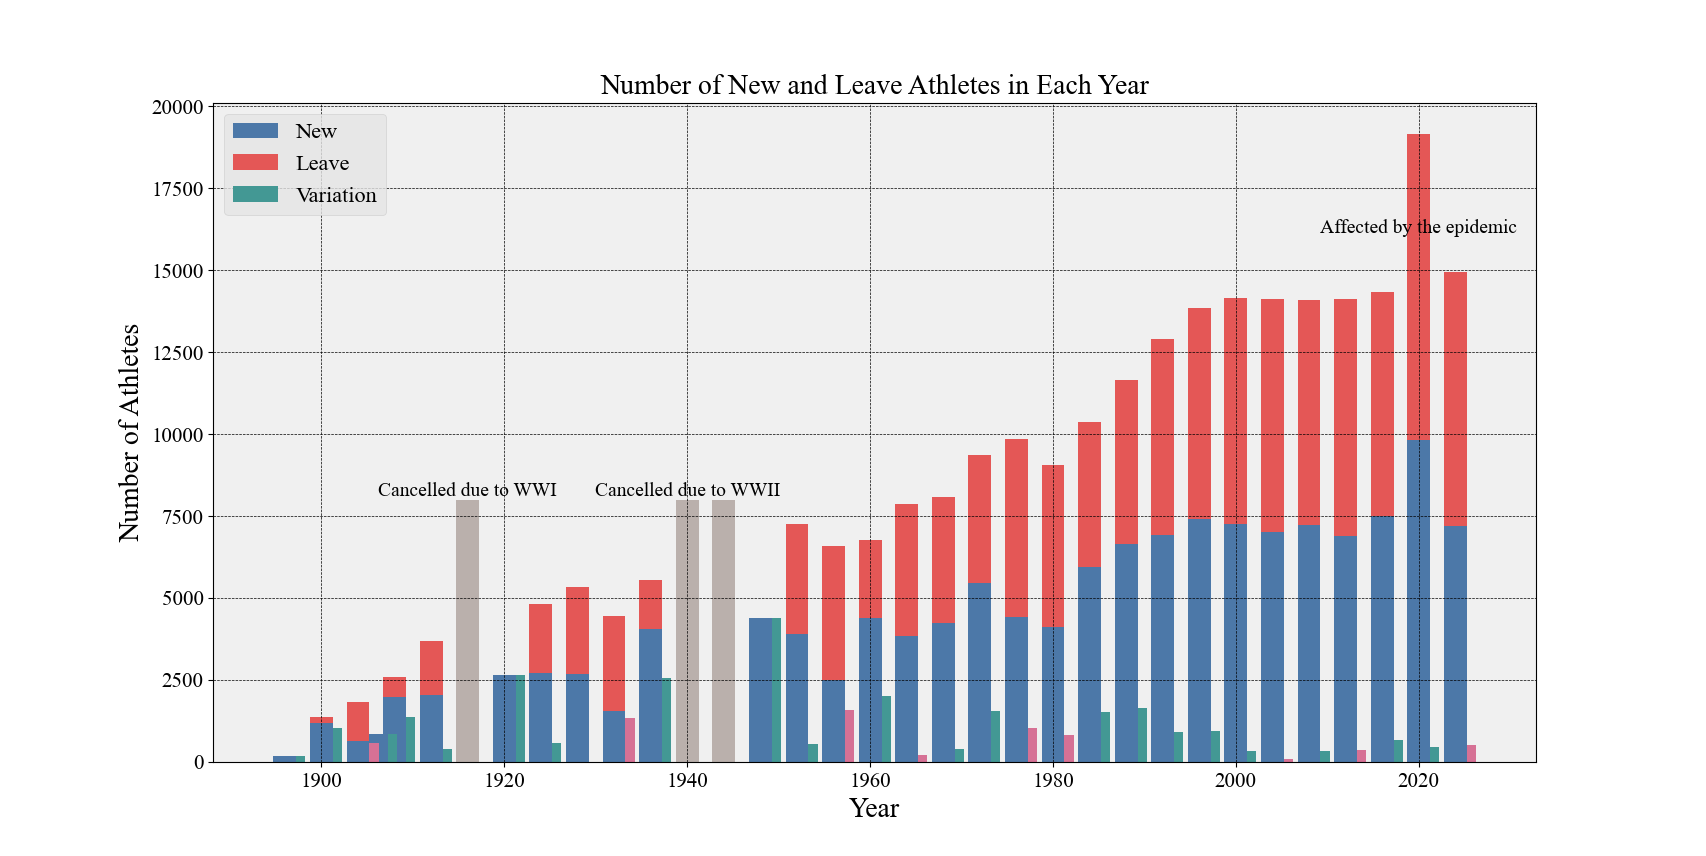
\includegraphics[width=12cm]{img/Number.png}
	\caption{Number of New and Leave Athletes in Each Year}
	\label{fig:aa}
\end{figure}

Then, we compiled the distribution of the times of participations and the distribution of athlete tenure based on historical data, as shown in the figure.
\begin{figure}[htbp]
	\centering
	\begin{subfigure}[b]{.55\textwidth}
		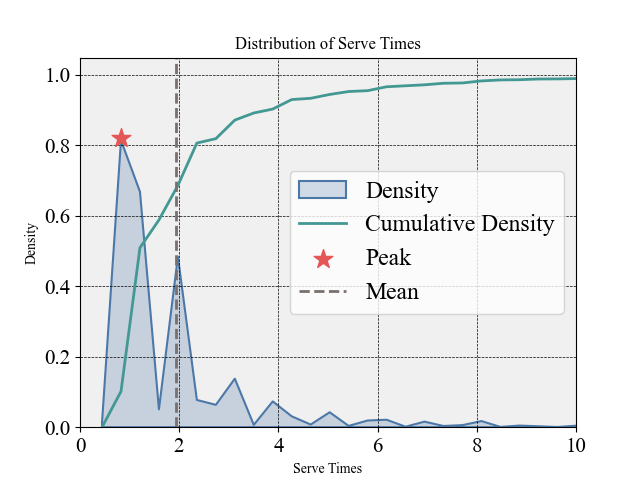
\includegraphics[width=\textwidth]{img/Times.png}
		\caption{Distribution of Serve Times}\label{subfig:left}
	\end{subfigure}
	\begin{subfigure}[b]{.4\textwidth}
		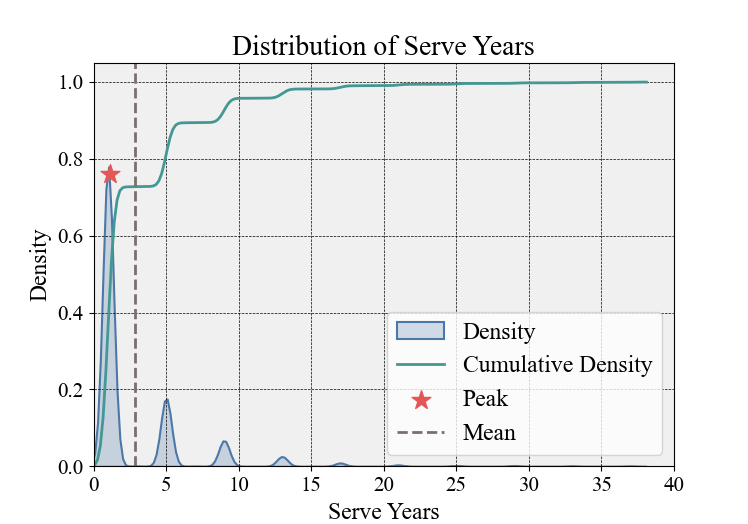
\includegraphics[width=\textwidth]{img/Years.png}
		\caption{Distribution of Serve Years}\label{subfig:right}
	\end{subfigure}
	\caption{Two images}\label{fig:subfigures}
\end{figure}


From the distribution chart, it can be seen that nearly 80% of athletes have participated in 1 or 2 matches, with the average number of serve times being 1.94, meaning each athlete participates in approximately 2 matches. Based on this assumption, we consider that each participating athlete will compete in 2 matches on average. Additionally, around 80% of athletes have participated in only 1 Olympic Games, while nearly 20% have participated in 2. Therefore, we can assume that 20% of the veteran athletes will continue to compete in the next Olympic Games, providing a basis for determining which athletes will continue to participate.

To predict the Participant List, we employed Monte Carlo simulation, which consisted of two parts: the first part involved selecting 20% of veteran athletes to continue competing (20% conforming to the original data distribution), while the second part generated new random athletes based on historical athlete data.

In the previous sections, we determined which athletes will continue to compete. To simulate new random athletes, we simplified each individual into three parameters: the probabilities of winning a gold, silver, or bronze medal.

For a given country in a specific event, the average number of medals won by all athletes serves as the standard number of medals for a representative athlete. The medal expectations were categorized into 3 scenarios: optimistic, moderate, and pessimistic. The optimistic expectation was calculated by averaging the top 50% of the team, the moderate expectation by averaging all team members, and the pessimistic expectation by averaging the bottom 50%. 

Using the Previous Participants' Records as the basis for Monte Carlo simulation, we ultimately determined the Participant List Prediction.



\subsubsection{Distribution of Countries' Strength Sports}
Due to factors such as cultural and geographical environments, countries exhibit distinct advantages in different events. For example, Kenya and Ethiopia excel in long-distance running, particularly in Athletics, largely due to the training conditions in high-altitude regions. Brazil, with its deep football culture, has produced many world-class players, a result of its warm climate and environment conducive to year-round outdoor sports.

By analyzing the performance of various countries in different events across past Olympic Games, we extracted a feature variable $\gamma$(Event Adeptness Coefficient), to represent the advantages of these countries in certain events..

%公式
\begin{equation}
	\gamma = \frac{m_{c_i,e_j}}{\sum m_{c_i,e_j}}
\end{equation}





By extracting features, we mined the level of expertise of each country in different events within the dataset, such as China's performance across various events, as shown in the figure below:

\begin{figure}[htbp]
	\centering
	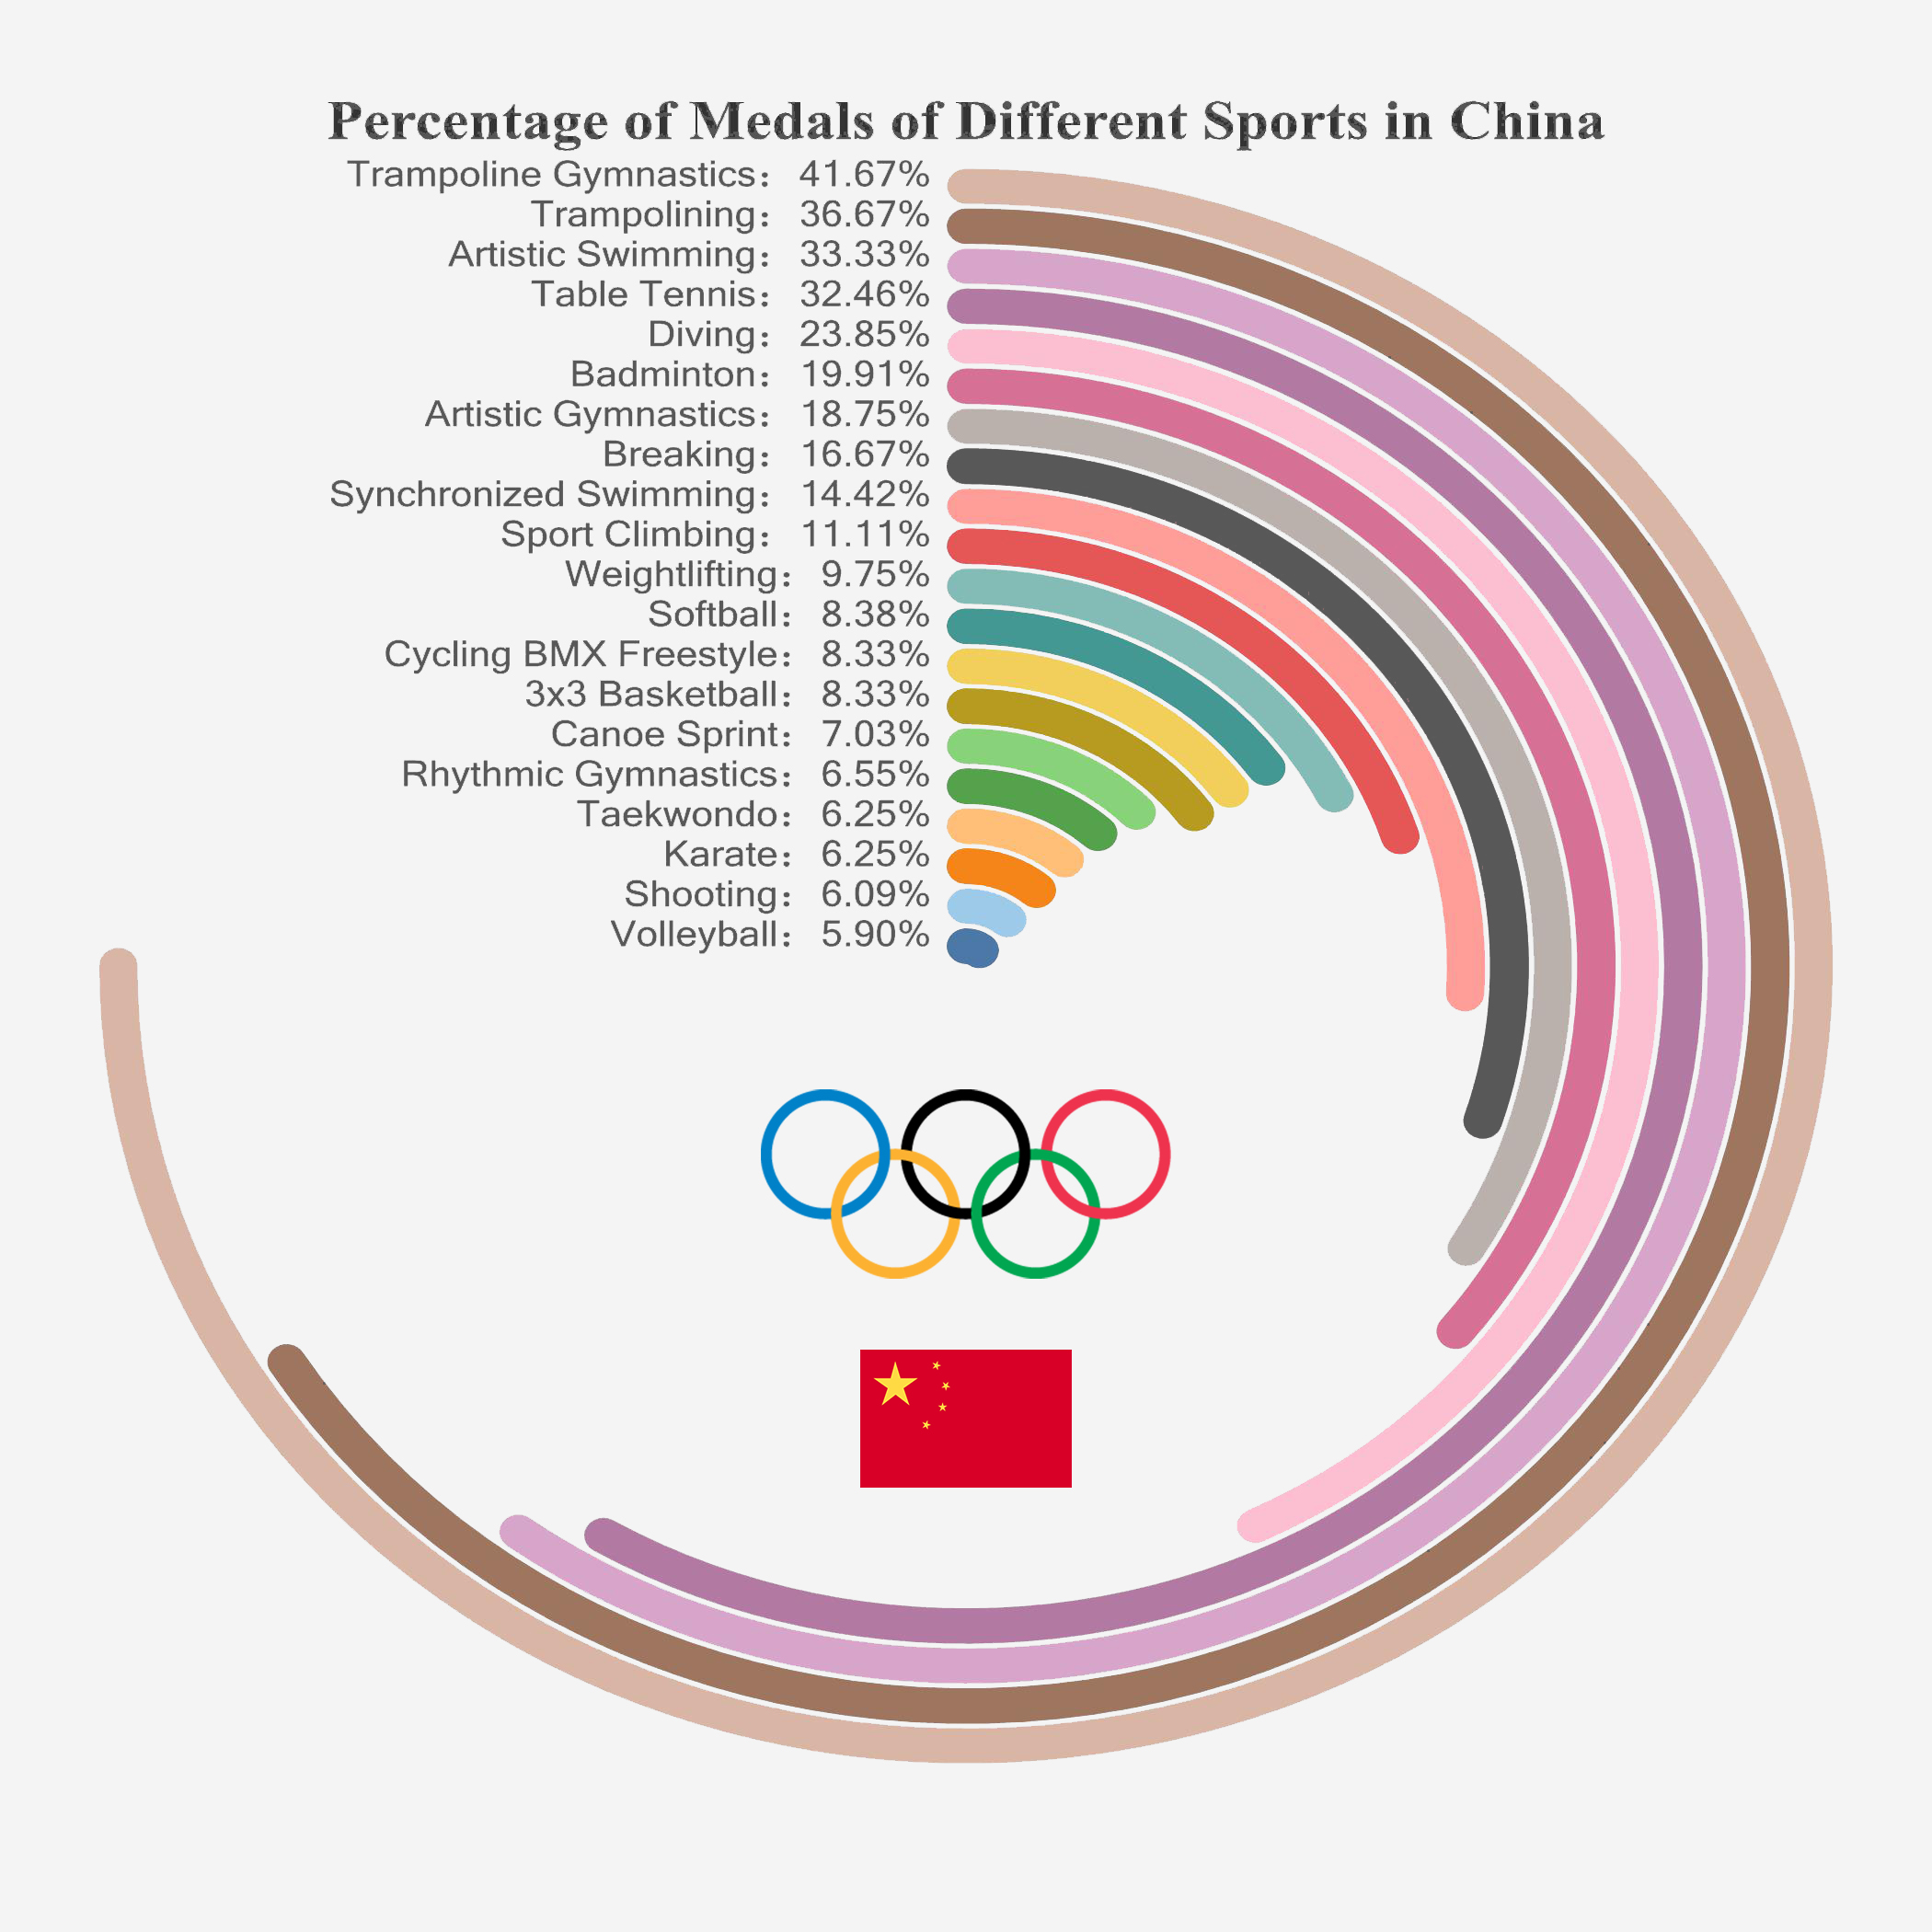
\includegraphics[width=12cm]{img/Percentage.jpg}
	\caption{Percentage of Medals of Different Sports in China}
	\label{fig:aa}
\end{figure}


\subsubsection{Changes in Medal Count}
Since the IOC makes adjustments to events each year, the total number of medals awarded in each event does not remain exactly the same each year. To address this, we applied \textbf Linear Regression to fit the number of gold, silver, and bronze medals awarded in each event across past Olympic Games and predicted the medal distribution for the upcoming Olympic Games, providing a reference for subsequent operations.

\section{Task1:Medal Prediction Model Based on LightGBM}
\subsection{Medal Standings}
Numerous factors influence the medal table. To predict the medal standings for the next Olympics, we incorporated factors identified during the data preprocessing stage, including nation level, the list of participating athletes, each country's adeptness in specific events, and adjustments to medal counts.

Additionally, as host countries typically benefit from home advantage, the factor of "whether a country is the host"or "whether hosting for the first time" was also considered. This factor was categorized into 3 categories and quantified for inclusion in the model. Ultimately, these five factors were collectively summarized as \textbf{National Background Factors}.

% \usepackage{longtable}


\begin{longtable}{|c|c|} 
	\hline
	Category & Definition               \endfirsthead 
	\hline
	0        & Not host                 \\ 
	\hline
	1        & Host for the 1st time    \\ 
	\hline
	2        & Host for more than once  \\
	\hline
\end{longtable}

The prediction of the Olympic medal table is essentially a multi-task learning problem, with the goal of predicting the number of gold, silver, and bronze medals each country is likely to win in different events. To accomplish this task, we need to input a large and diverse set of data while outputting predictions for multiple medal categories. These features are highly suitable for the LightGBM model.

Building on GBDT, LightGBM accelerates the computation using histograms, optimizing training efficiency and enabling the fast processing of high-dimensional, sparse, large-scale data. Compared to traditional logistic regression, LightGBM can capture nonlinear relationships through tree splitting, offering a performance advantage in accurately handling complex data and nonlinear relationships, significantly improving accuracy. Additionally, it can automatically handle missing values, providing great convenience for data preprocessing.

As a gradient boosting-based regression model, in LightGBM, the objective function consists of two parts: the loss function and the regularization term.

\begin{equation}
	\mathcal{L} = \sum_{i=1}^{n} L(y_i, \hat{y}_i^{(m-1)} + \eta f_m(x_i)) + \Omega(f_m)
\end{equation}
The optimized loss function based on GBDT is represented as squared error in the medal prediction regression task.

$y_i$denotes the true value.
$\hat{y}_i^{(m-1)}$is the current model's predicted value.
$\hat{y}_i^{(m-1)}$+$\eta f_m(x_i)$is the model's predicted value at the m-th step during the gradient boosting model update process.
$\Omega(f_m)$ Regularization term, which prevents overfitting of the model and controls the complexity of the trees.

We input the previously obtained data into LightGBM for iterative model training. After training, we input the factors affecting the predictions for the next edition into the model, ultimately obtaining the predicted medal table for the 2028 Summer Olympics in Los Angeles, USA, as follows:
%奖牌榜预测图
\begin{figure}[htbp]
	\centering
	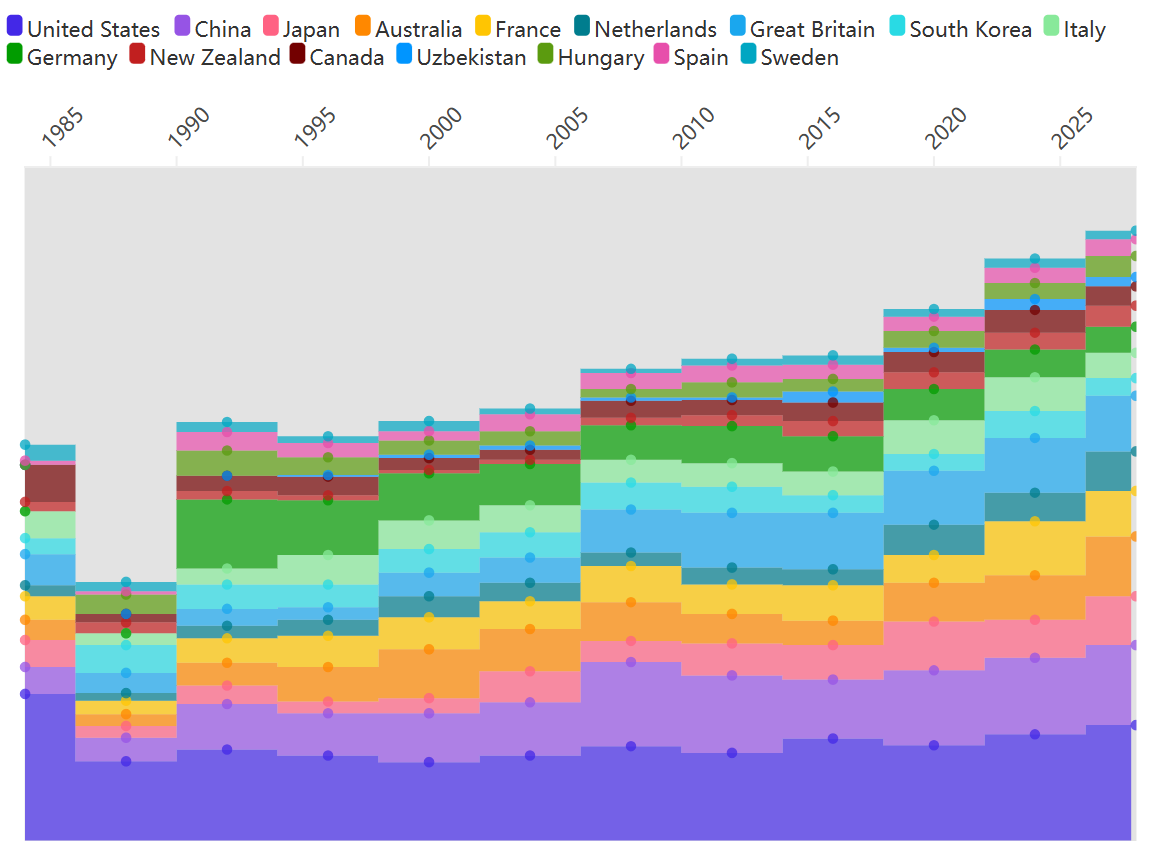
\includegraphics[width=12cm]{img/Predict.png}
	\caption{Medal count prediction}
	\label{fig:aa}
\end{figure}
According to the model's predictions, the United States is expected to see a significant increase in medal count compared to the previous year, while France will experience a notable decrease, which is related to the home-field advantage of the host country. Additionally, due to changes in the number of medals for certain events, the medal counts for Australia, Japan, and the Netherlands are expected to rise, while Italy and South Korea will see a decline. China's medal count is projected to remain relatively stable.

To more accurately simulate the actual number of medals won, we simplify each individual into 3 parameters: the probabilities of winning gold, silver, and bronze medals. For a specific country and event, the average number of medals won by all team members represents the probability that a standard "virtual athlete" should have.

For the expected outcomes, the optimistic expectation is calculated by averaging the top 50% of the team, the moderate expectation is based on the average of all team members, and the pessimistic expectation is derived by averaging the bottom 50% of the team.

The "Previous Participants Record" serves as the basis for the Monte Carlo simulation, which consists of two parts: the first part involves selecting 20% of veteran athletes to continue competing (with 20% corresponding to the original data distribution), and the second part uses historical athlete data to generate new random athletes.







Based on the model, we predict the medal outcomes for each country in the 2028 Olympic Games. A partial result is provided here, with the full version available in the appendix. The predicted outcomes for the United States are presented, showing that, overall, the optimistic expectation > moderate expectation > pessimistic expectation. 
\begin{longtable}{l|c|c|c|c|c|c|c|c|c|c}
\caption{Countries' Medal Count Prediction(part)}\\
	Country              & \multicolumn{1}{l|}{\begin{tabular}[c]{@{}l@{}}G\_\\pes.\end{tabular}} & \multicolumn{1}{l|}{\begin{tabular}[c]{@{}l@{}}S\_\\pes.\end{tabular}} & \multicolumn{1}{l|}{\begin{tabular}[c]{@{}l@{}}B\_\\pes.\end{tabular}} & \multicolumn{1}{l|}{\begin{tabular}[c]{@{}l@{}}G\_\\opt.\end{tabular}} & \multicolumn{1}{l|}{\begin{tabular}[c]{@{}l@{}}S\_\\opt.\end{tabular}} & \multicolumn{1}{l|}{\begin{tabular}[c]{@{}l@{}}B\_\\opt.\end{tabular}} & \multicolumn{1}{l|}{Gold} & \multicolumn{1}{l|}{Silver} & \multicolumn{1}{l|}{Bronze} & \multicolumn{1}{l}{Total}  \endfirsthead 
	\hline
	United States        & 47                                                                     & 36                                                                     & 23                                                                     & 53                                                                     & 41                                                                     & 25                                                                     & 51                        & 40                          & 25                          & 117                        \\ 
	\hline
	China                & 35                                                                     & 35                                                                     & 15                                                                     & 46                                                                     & 38                                                                     & 20                                                                     & 40                        & 36                          & 17                          & 95                         \\ 
	\hline
	Australia            & 28                                                                     & 20                                                                     & 22                                                                     & 33                                                                     & 24                                                                     & 24                                                                     & 29                        & 22                          & 23                          & 71                         \\ 
	\hline
	France               & 23                                                                     & 19                                                                     & 19                                                                     & 27                                                                     & 20                                                                     & 22                                                                     & 24                        & 19                          & 21                          & 64                         \\ 
	\hline
	Germany              & 18                                                                     & 24                                                                     & 14                                                                     & 23                                                                     & 26                                                                     & 16                                                                     & 21                        & 25                          & 15                          & 61                         \\ 
	\hline
	United Kingdom       & 20                                                                     & 19                                                                     & 14                                                                     & 26                                                                     & 24                                                                     & 15                                                                     & 25                        & 21                          & 15                          & 61                         \\ 
	\hline
	Japan                & 16                                                                     & 25                                                                     & 14                                                                     & 19                                                                     & 27                                                                     & 16                                                                     & 17                        & 26                          & 16                          & 58                         \\ 
	\hline
	Italy                & 15                                                                     & 20                                                                     & 15                                                                     & 17                                                                     & 20                                                                     & 22                                                                     & 16                        & 20                          & 16                          & 53                         \\ 
	\hline
	Spain                & 21                                                                     & 10                                                                     & 13                                                                     & 30                                                                     & 12                                                                     & 14                                                                     & 25                        & 12                          & 13                          & 50                         \\ 
	\hline
	Netherlands          & 24                                                                     & 6                                                                      & 13                                                                     & 29                                                                     & 9                                                                      & 15                                                                     & 26                        & 8                           & 15                          & 47                         \\ 
	\hline
	New Zealand          & 20                                                                     & 13                                                                     & 9                                                                      & 22                                                                     & 15                                                                     & 10                                                                     & 22                        & 14                          & 9                           & 45                         \\ 
	\hline
	...                  & ..                                                                     & ..                                                                     & ..                                                                     & ..                                                                     & ..                                                                     & ..                                                                     & ..                        & ..                          & ..                          & ..                         \\
	\multicolumn{1}{l}{} & \multicolumn{1}{c}{}                                                   & \multicolumn{1}{c}{}                                                   & \multicolumn{1}{c}{}                                                   & \multicolumn{1}{c}{}                                                   & \multicolumn{1}{c}{}                                                   & \multicolumn{1}{c}{}                                                   & \multicolumn{1}{c}{}      & \multicolumn{1}{c}{}        & \multicolumn{1}{c}{}        &                           
\end{longtable}
%4.2
\subsection{Countries that Win Their First Medal}
Since the model used for predicting the medal table in the previous section yields varying levels of accuracy for countries of different rankings, the predictions for higher-ranked countries, such as the United States and China, are more accurate. In contrast, the prediction errors for lower-ranked countries are larger. Clearly, countries that have not yet won medals fall into the category with higher prediction errors, so the previous model is not applicable in this case.

Therefore, for countries that have never won a medal before, we calculate their first medal index $\xi$.
%公式 未知







The number of competitions is counted from the original dataset, and the expected increase in the number of medals for the next edition is predicted through a Linear Regression model based on historical data.

As the number of competitions and the expected increase in medals for the next edition increase for countries that have not won medals, the likelihood of these countries winning medals becomes higher. Therefore, the first medal index $\xi$ is positively correlated with the probability of a country that has not won a medal securing its first medal in the next Olympic Games, meaning that the larger the $\xi$ value, the higher the likelihood of winning the first medal.

In order to visualize the accuracy of a country's first medal prediction, we normalized the first medal index using the Z-score and then multiplied it by 0.8 to obtain the first medal coefficient $\kappa$.

\begin{equation}
	\kappa = 0.8 \times \frac{\xi - \overline{\xi}}{\sigma}
\end{equation}
Here,$\overline{\xi}$ refers to the mean of the original data, and$\sigma$refers to the standard deviation of the original data.
The calculated results are as follows:
%首奖可能性图
\begin{figure}[htbp]
	\centering
	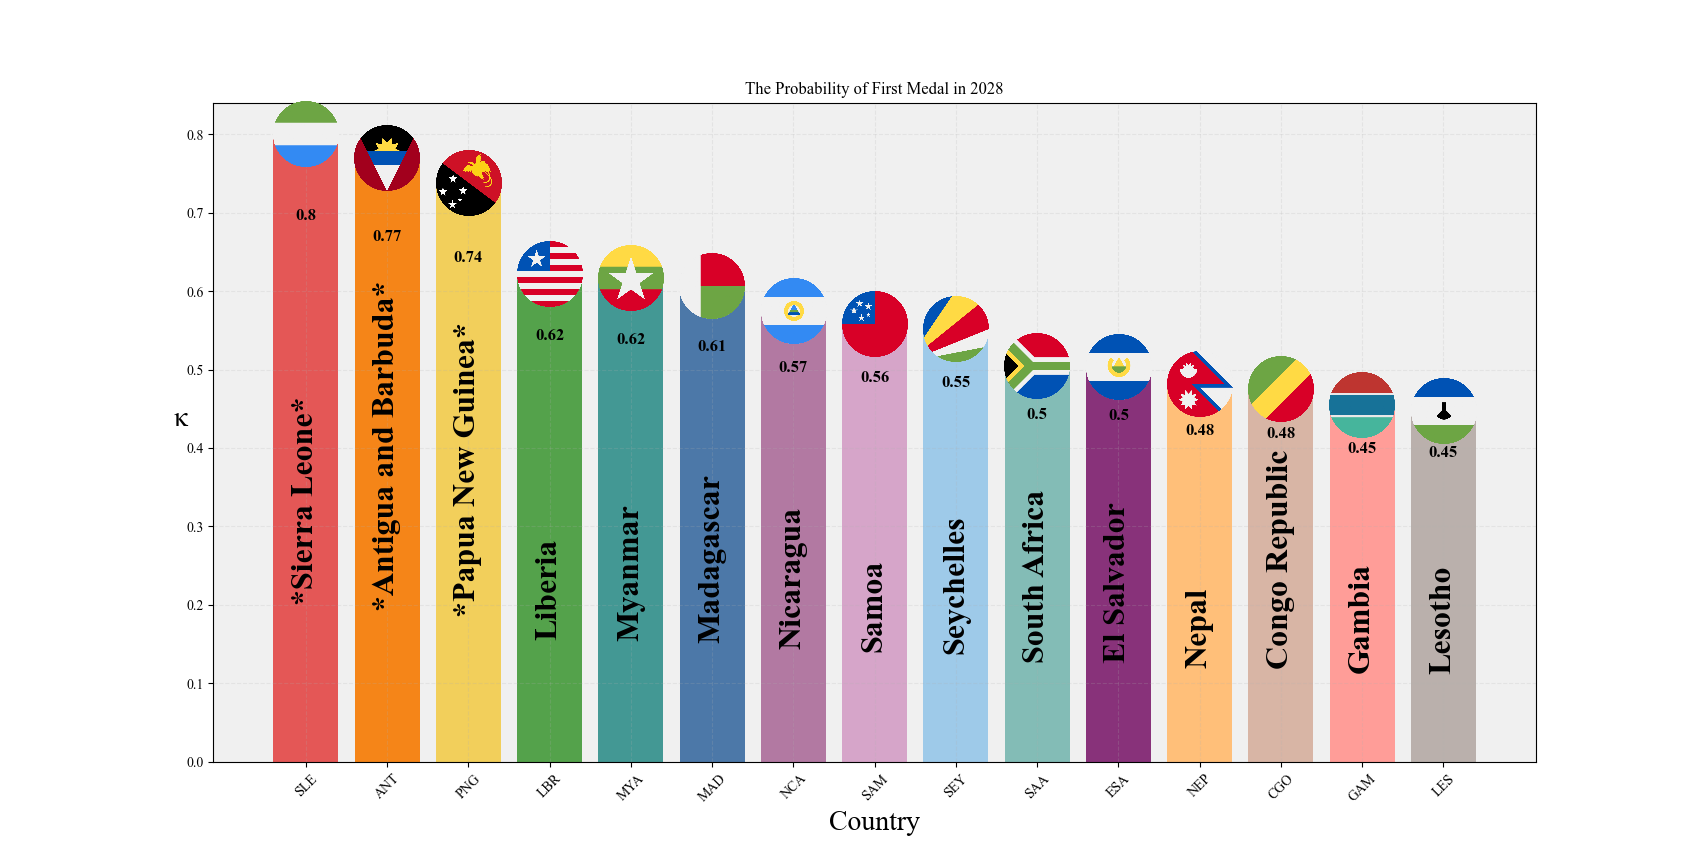
\includegraphics[width=16cm]{img/First.png}
	\caption{The Probability of First Medal in 2028}
	\label{fig:aa}
\end{figure}


As shown in the figure, Sierra Leone (SLE), Antigua and Barbuda (ANT), and Papua New Guinea (PNG) are the three countries most likely to win their first medal in the next Olympic Games, with accuracies approximately 0.8, 0.77, and 0.74, respectively.


%4.3
\subsection{Events and Medal Counts by Countries}
In the data preprocessing section, we have calculated the adeptness of each country in each event, thus allowing us to roughly estimate the events in which each country excels.

We input the data of the dominant events of multiple countries into the prediction model and use \textbf{Spearman's Rank Correlation Coefficient} to analyze the correlation between the total medal count of a country and the medal count of a specific event, as well as the number of events in that event. This is because we cannot confirm that the data sample follows a normal distribution, nor can we ascertain that the relationship between the dominant events and the total medal count is linearly correlated. Spearman's Rank Correlation Coefficient is suitable for evaluating \textbf{nonlinear} relationships.

We studied the relationship between China's total medal count, gold medal count, and the number of awards and events in table tennis. For each pair of variables, we ranked the data points and assigned ranks to each data point. The rank difference for each data point is calculated as:

\begin{equation}
	d_i = R(X_i) - R(Y_i)
\end{equation}

\begin{equation}
	R_s = 1 - \frac{6 \sum d_i^2}{n(n^2 - 1)}
\end{equation}


Here, $d_i$ is the rank difference of the two variables for the iii-th data point. 
Next, we compute the Spearman's Rank Correlation Coefficient ($R_s$). 

The absolute value of $R_s$ closer to 1 indicates a stronger correlation, while closer to 0 indicates a weaker correlation.A positive $R_s$ indicates a positive correlation between the two variables, meaning an increase in one variable typically accompanies an increase in the other. 

Through extensive data analysis, we identified 3 typical examples: table tennis in China, Athletics in Jamaica, and rowing in New Zealand, as shown in the figure.
%三个国家擅长项目的图
\begin{figure}[htbp]
	\centering
	\begin{subfigure}[b]{.3\textwidth}
		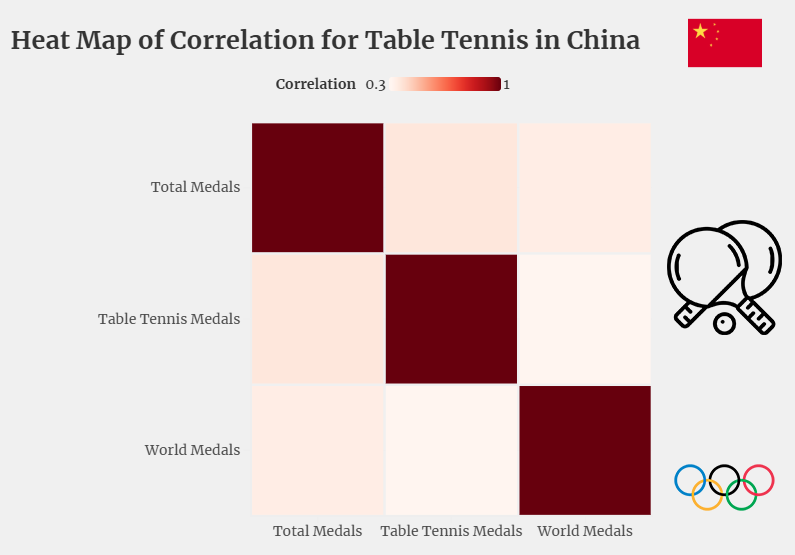
\includegraphics[width=\textwidth]{img/Table Tennis.png}
		\caption{Heatmap of Correlation for Table Tennis in China}\label{subfig:1}
	\end{subfigure}
	\hfill 
	\begin{subfigure}[b]{.33\textwidth}
		
\includegraphics[width=\textwidth]{img/Jamaica.png}
		\caption{ Heatmap of Correlation for Athletics in Jamaica}\label{subfig:2}
	\end{subfigure}
	\hfill 
	\begin{subfigure}[b]{.32\textwidth}
		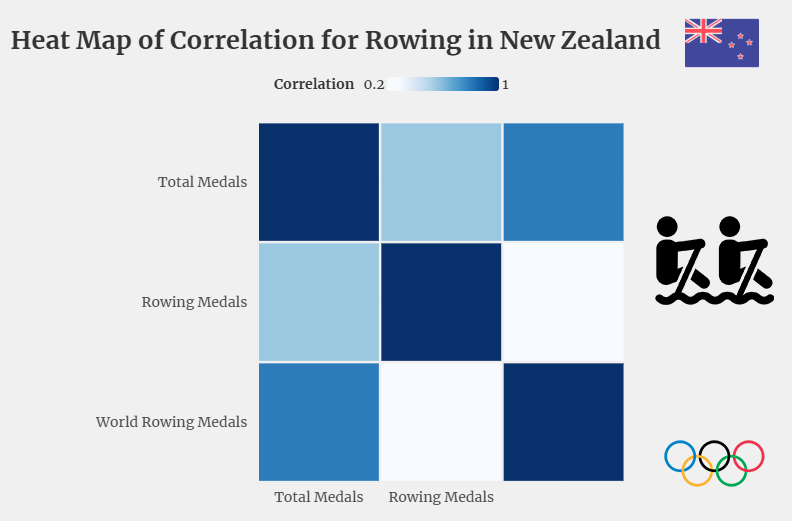
\includegraphics[width=\textwidth]{img/New Zealand.png}
		\caption{Heatmap of Correlation for Rowing in New Zealand}\label{subfig:3}
	\end{subfigure}
	\caption{Three images}\label{fig:subfigures}
\end{figure}

We found that although China has a significant advantage in table tennis, the relationship between the development of the event and China's total medal count is relatively weak. This suggests that China's overall athletic adeptness is stable and less influenced by a single dominant event.

Additionally, Jamaica's total medal count shows a strong positive correlation with its performance in athletics, indicating the country's heavy reliance on athletics competitions. Since athletics is a well-established and stable event with minimal fluctuations in the number of events held each year, the relationship between the number of events and Jamaica's total medal count is relatively weak. 

New Zealand also has a high dependency on rowing, with a substantial portion of its medals coming from this event. However, unlike Jamaica, rowing is not as established as athletics, and the number of competitions fluctuates from year to year. As a result, New Zealand's overall medal count is highly dependent on the rise and fall of rowing's prominence.
\subsection{Model Performances}

We calculated four evaluation metrics: Mean Squared Error (MSE), Root Mean Squared Error (RMSE), Mean Absolute Error (MAE), and the Coefficient of Determination (\(\mathbf{R}^2\)).

Among these, smaller values for the first three metrics and a larger value for R² indicate better model performance.

% \usepackage{longtable}

\begin{longtable}{l|l|l|l|l} 
	\caption{Model Performances(LightGBM)}\\ 
	\hline
	\multicolumn{1}{c|}{\textbf{Model}} & \multicolumn{1}{c|}{\textbf{MSE}} & \multicolumn{1}{c|}{\textbf{RMSE}} & \multicolumn{1}{c|}{\textbf{MAE}} & \multicolumn{1}{c}{\(\mathbf{R}^2\)}  \endfirsthead 
	\hline
	Gold Prediction                     & 0.0235                            & 0.180                              & 0.030                             & 0.890                              \\ 
	\hline
	Silver Prediction                   & 0.0239                            & 0.185                              & 0.033                             & 0.825                              \\ 
	\hline
	Bronze Prediction                   & 0.0231                            & 0.187                              & 0.034                             & 0.806                              \\
	\hline
\end{longtable}


%雷达图
\begin{figure}[htbp]
	\centering
	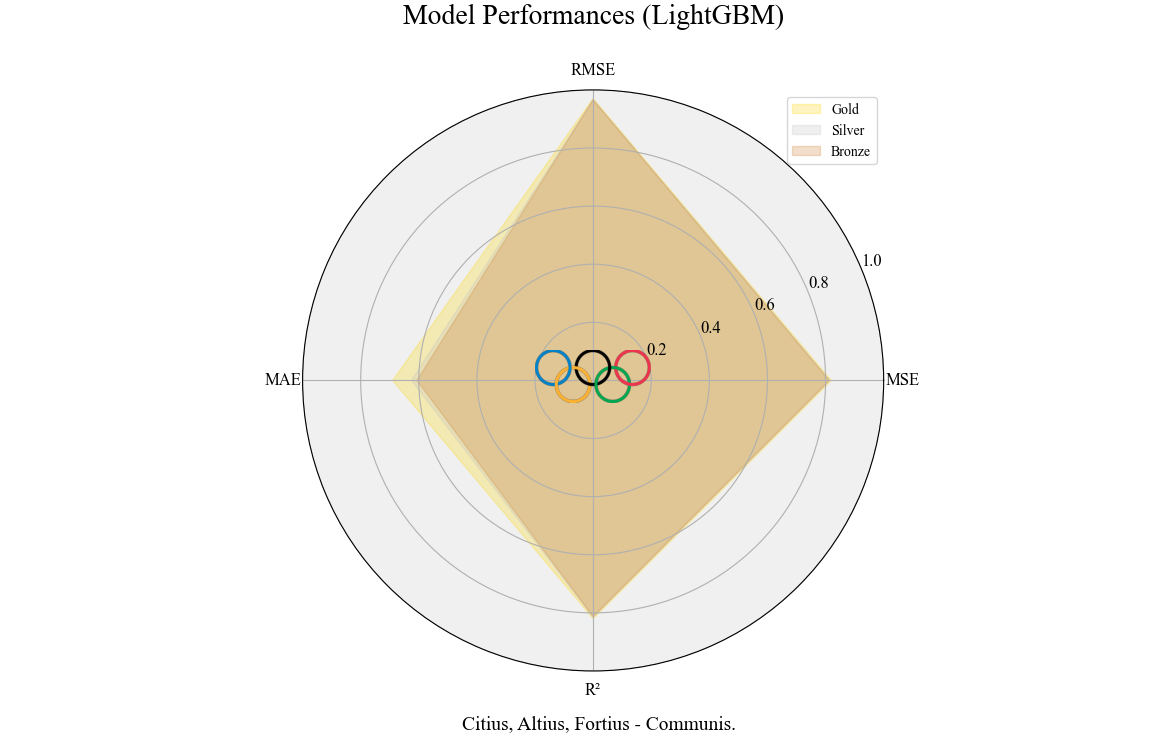
\includegraphics[width=8cm]{img/Performance.png}
	\caption{Model Performance Radar Chart}
	\label{fig:aa}
\end{figure}


It can be observed that the evaluation metrics for the prediction of the 3 types of medals show good performance with relatively small differences. 

A comparison reveals that the model's prediction accuracy for gold medals is relatively higher, with the highest \(\mathbf{R}^2\) and the lowest Root Mean Squared Error (RMSE) and Mean Absolute Error (MAE).



%5.1 排球
\begin{figure}[htbp]
	\centering
	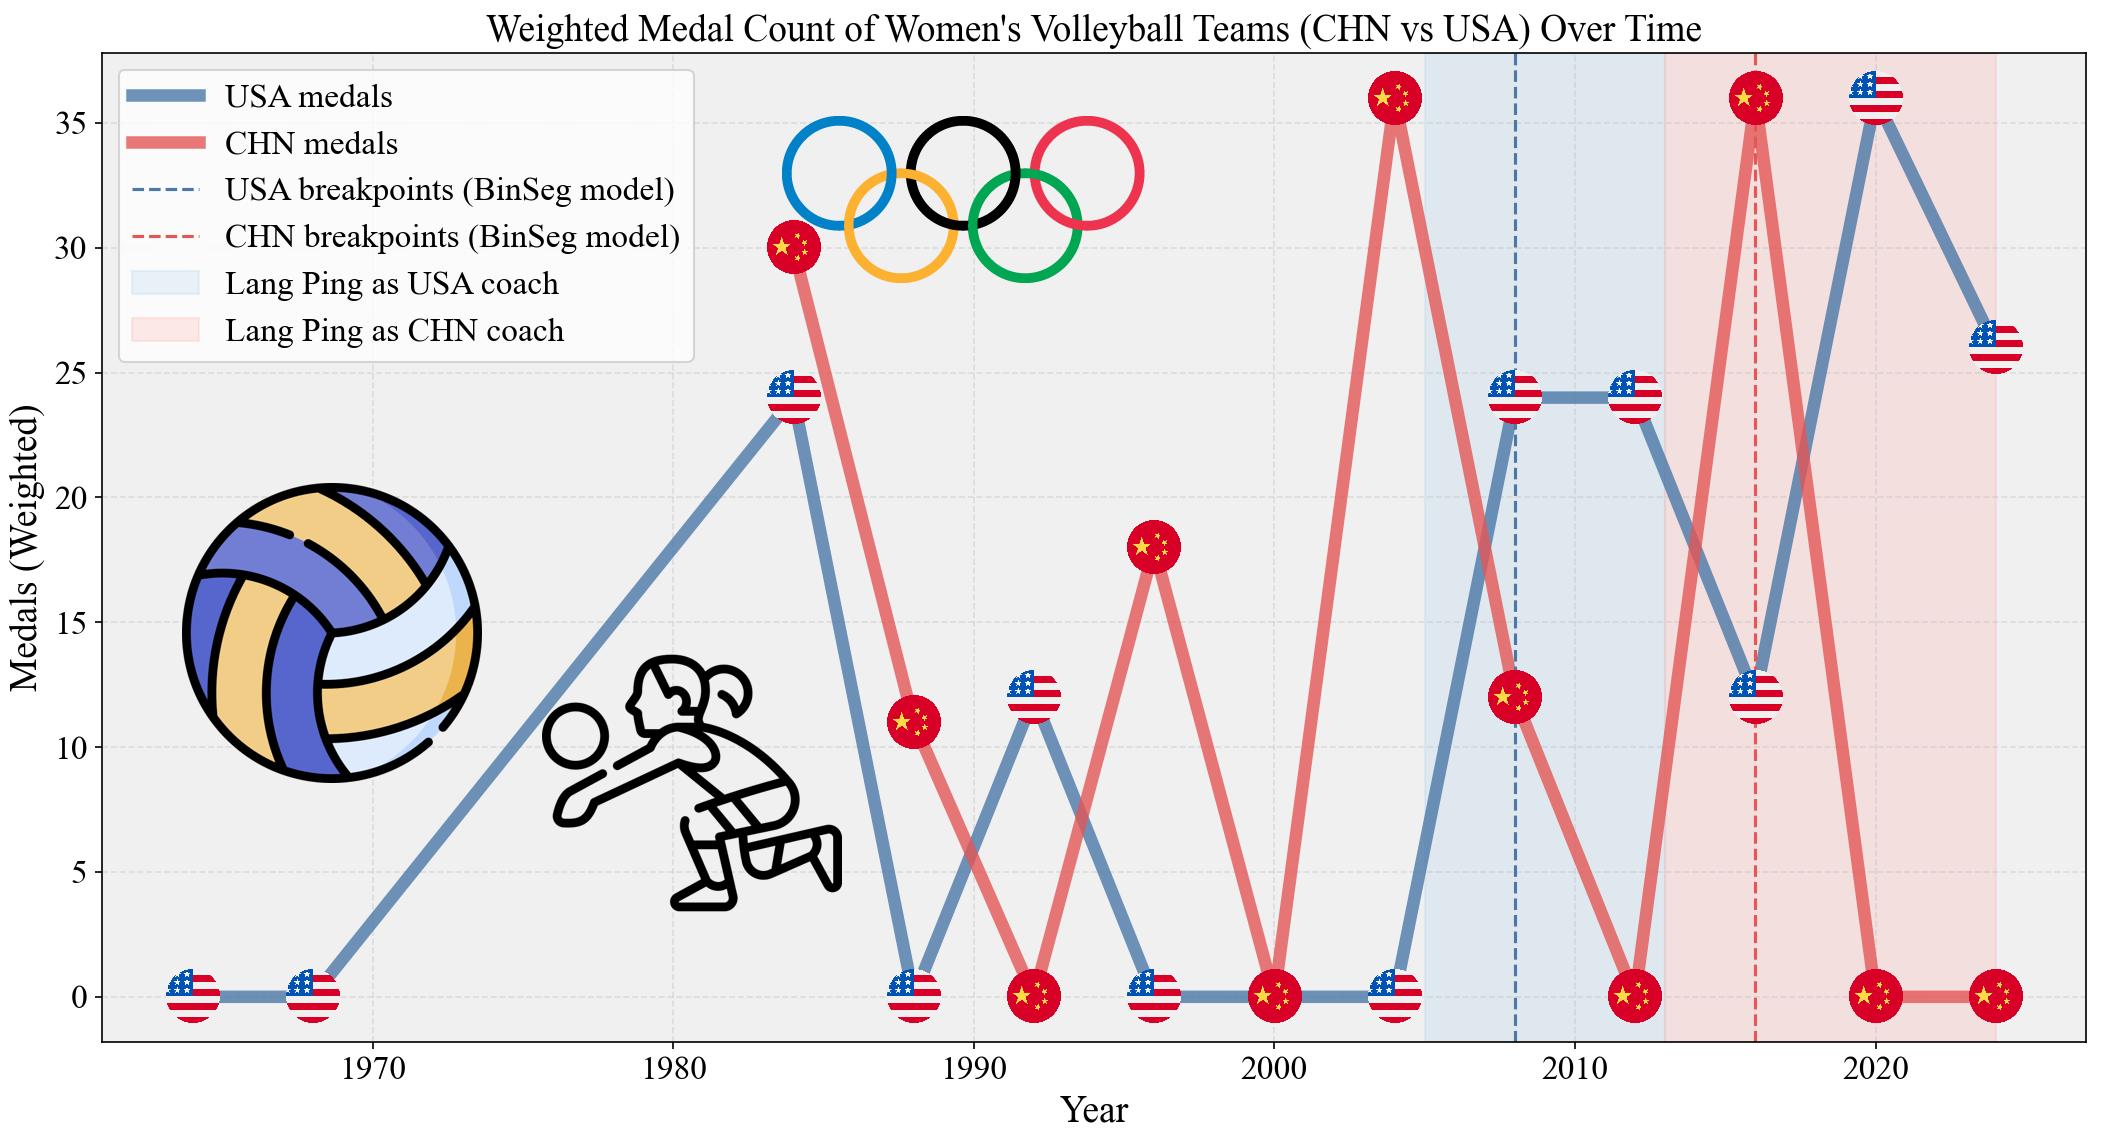
\includegraphics[width=12cm]{img/Volleyball.png}
	\caption{Medal Count of Women's Volleyball Teams(CHN vs USA) Over Time}
	\label{fig:aa}
\end{figure}

%三个国家某项目衰弱 需要教练图
\begin{figure}[htbp]
	\centering
	\begin{subfigure}[b]{.32\textwidth}
		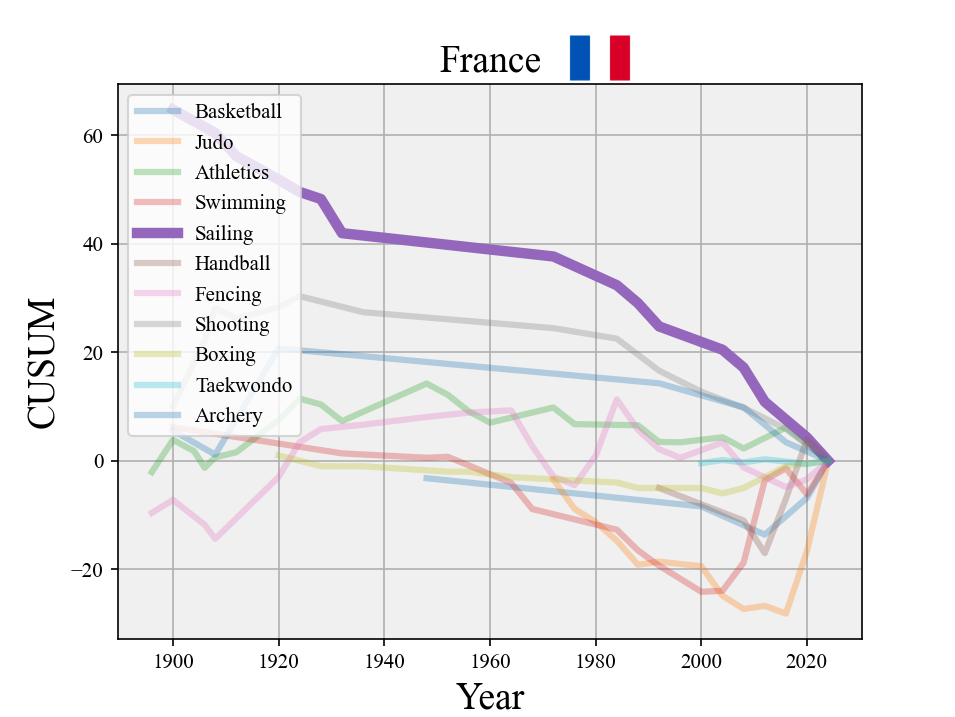
\includegraphics[width=\textwidth]{img/Decline1.png}
		\caption{France}\label{subfig:1}
	\end{subfigure}
	\hfill 
	\begin{subfigure}[b]{.32\textwidth}
		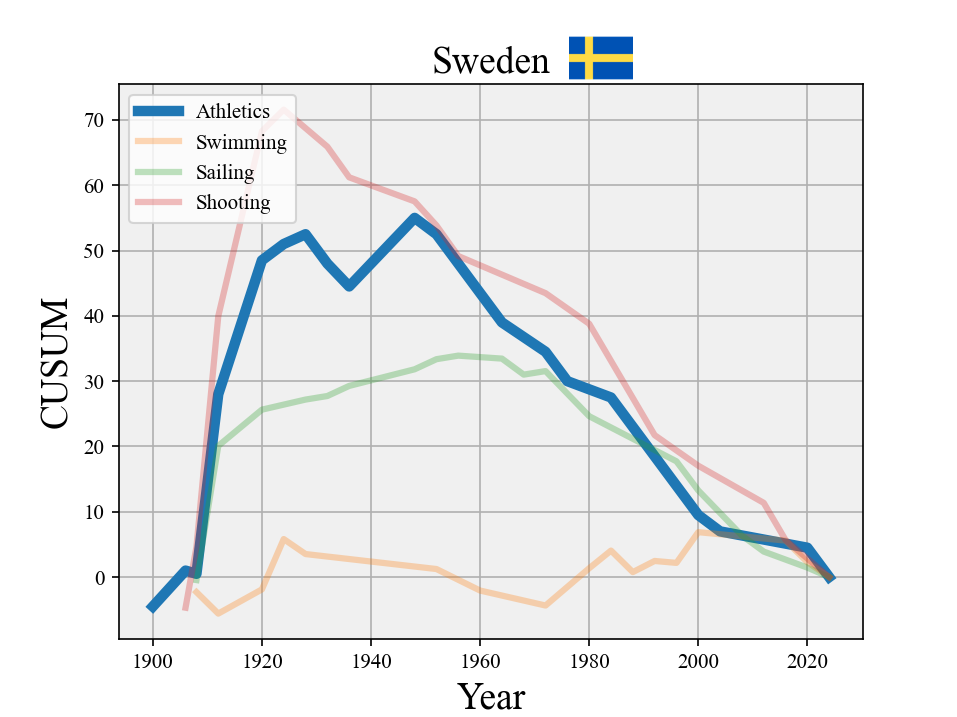
\includegraphics[width=\textwidth]{img/Decline2.png}
		\caption{Sweden}\label{subfig:2}
	\end{subfigure}
	\hfill 
	\begin{subfigure}[b]{.32\textwidth}
		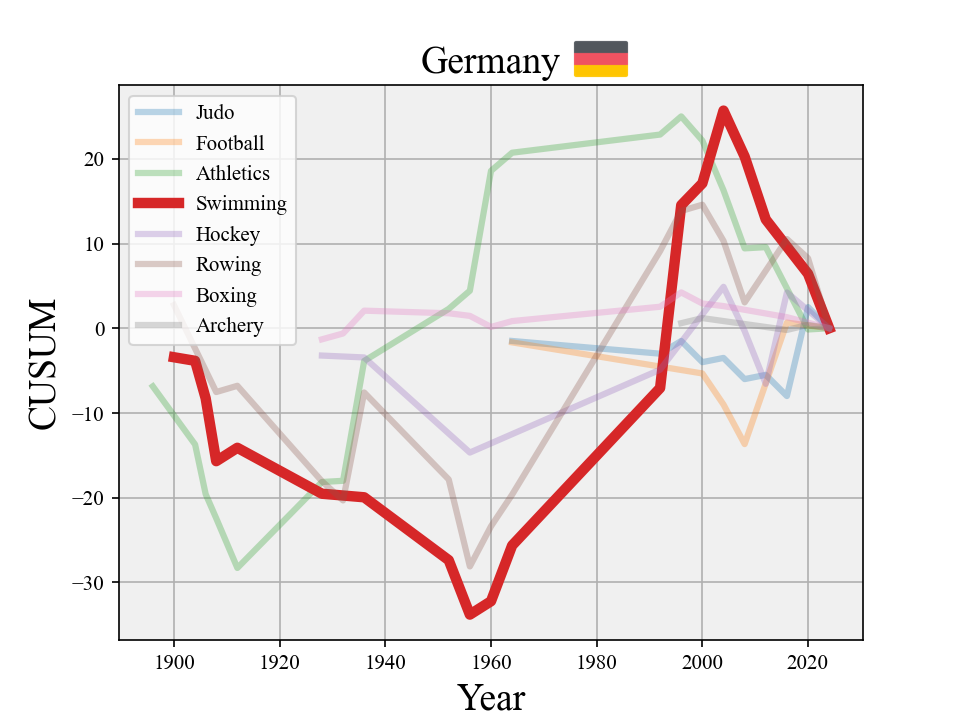
\includegraphics[width=\textwidth]{img/Decline3.png}
		\caption{Germany}\label{subfig:3}
	\end{subfigure}
	\caption{Three images}\label{fig:subfigures}
\end{figure}



%引用图像示例Figure \ref{fig:subfigures}
%Figure \ref{fig:subfigures} gives an example of subfigures. Figure \ref{subfig:left} is on the left, and Figure \ref{subfig:right} is on the right.




\begin{figure}[htbp]
	\centering
	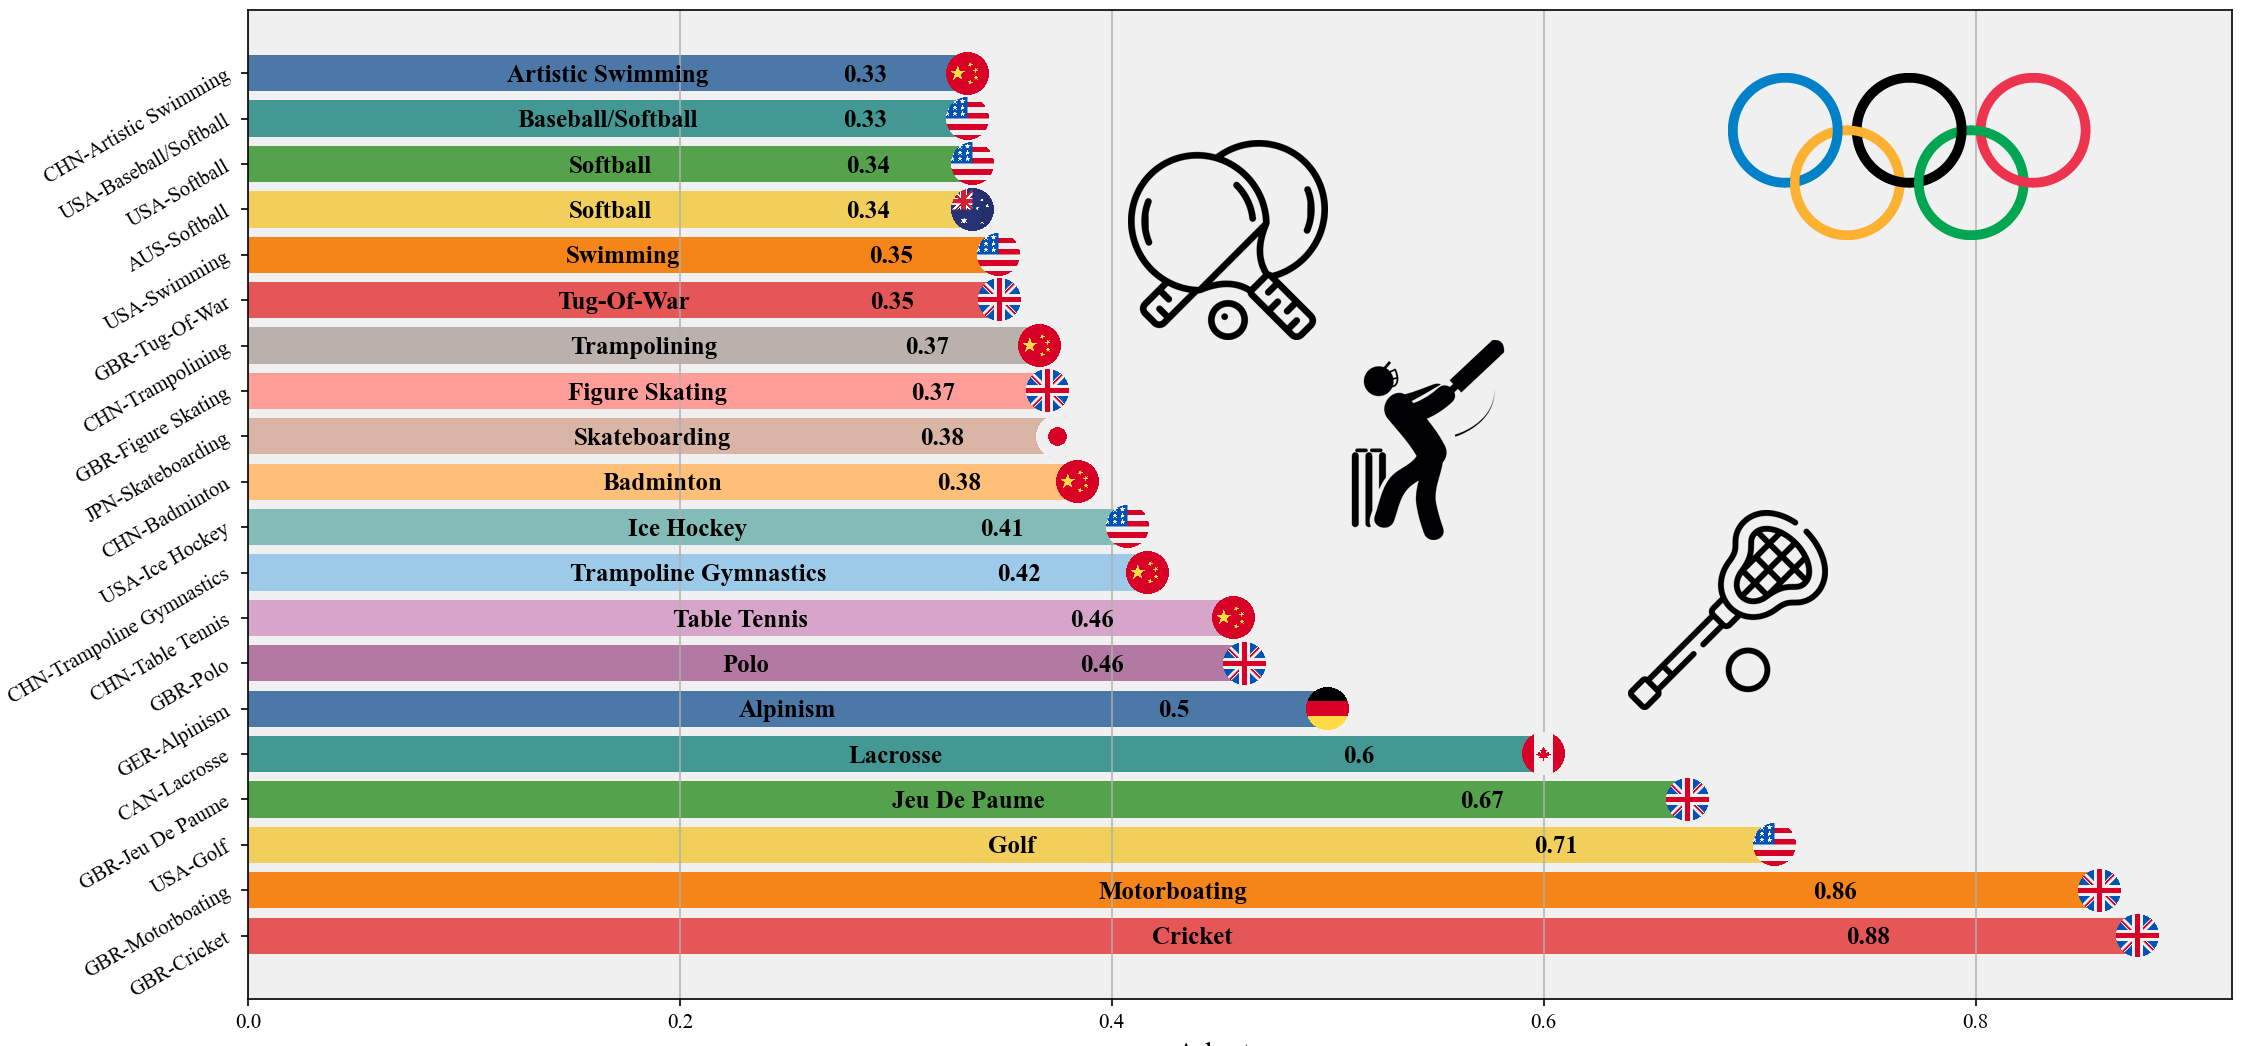
\includegraphics[width=16cm]{img/Monopolized Sports.png}
	\caption{Adeptness of Countries in Specitific Project}
	\label{fig:aa}
\end{figure}

\section{Task2:A "Great Coach" Effect}





\section{Verification of the "Great Coach" Effect}
The "Great Coach" effect can cause significant differences in the performance of relevant countries in corresponding events. To collect evidence of changes caused by this effect, we use a Bayesian Changepoint Detection (BEAST) model.

The BEAST model uses Bayesian inference to calculate the posterior probabilities of changes occurring at different time points, determining which time points are potential change points.


	
In the time series dataset \(X = (x_1, x_2, x_3, \ldots, x_T)\), we identify the set of change points \(C = \{c_1, c_2, \ldots, c_K\}\), where each \(c_k\) represents a change point.
Using Bayes' theorem, we can compute the posterior probability for each possible change point $c_k$:

\begin{equation}
	P(c_k \mid X) = \frac{P(X \mid c_k) P(c_k)}{P(X)}
\end{equation}
In this case, \( P(X|c_k) \) represents the likelihood of the data at the change point \( c_k \), \( P(c_k) \) is the prior probability, and \( P(X) \) is the marginal likelihood of the data.

\section{Task3}

%公式代码集合

	




\begin{equation}
	C_t^+ = \max(0, C_{t-1}^+ + (X_t - \mu - k))
\end{equation}
$C_t^+ $







	
	\begin{equation}
		\phi_i(f) = \sum_{S \subseteq N \setminus \{i\}} \frac{|S|!(|N| - |S| - 1)!}{|N|!} [f(S \cup \{i\}) - f(S)]
	\end{equation}



$\phi_i(f)$

%6.1
\subsection{Global Geopolitics}

%6.1 男女比例图
\begin{figure}[htbp]
	\centering
	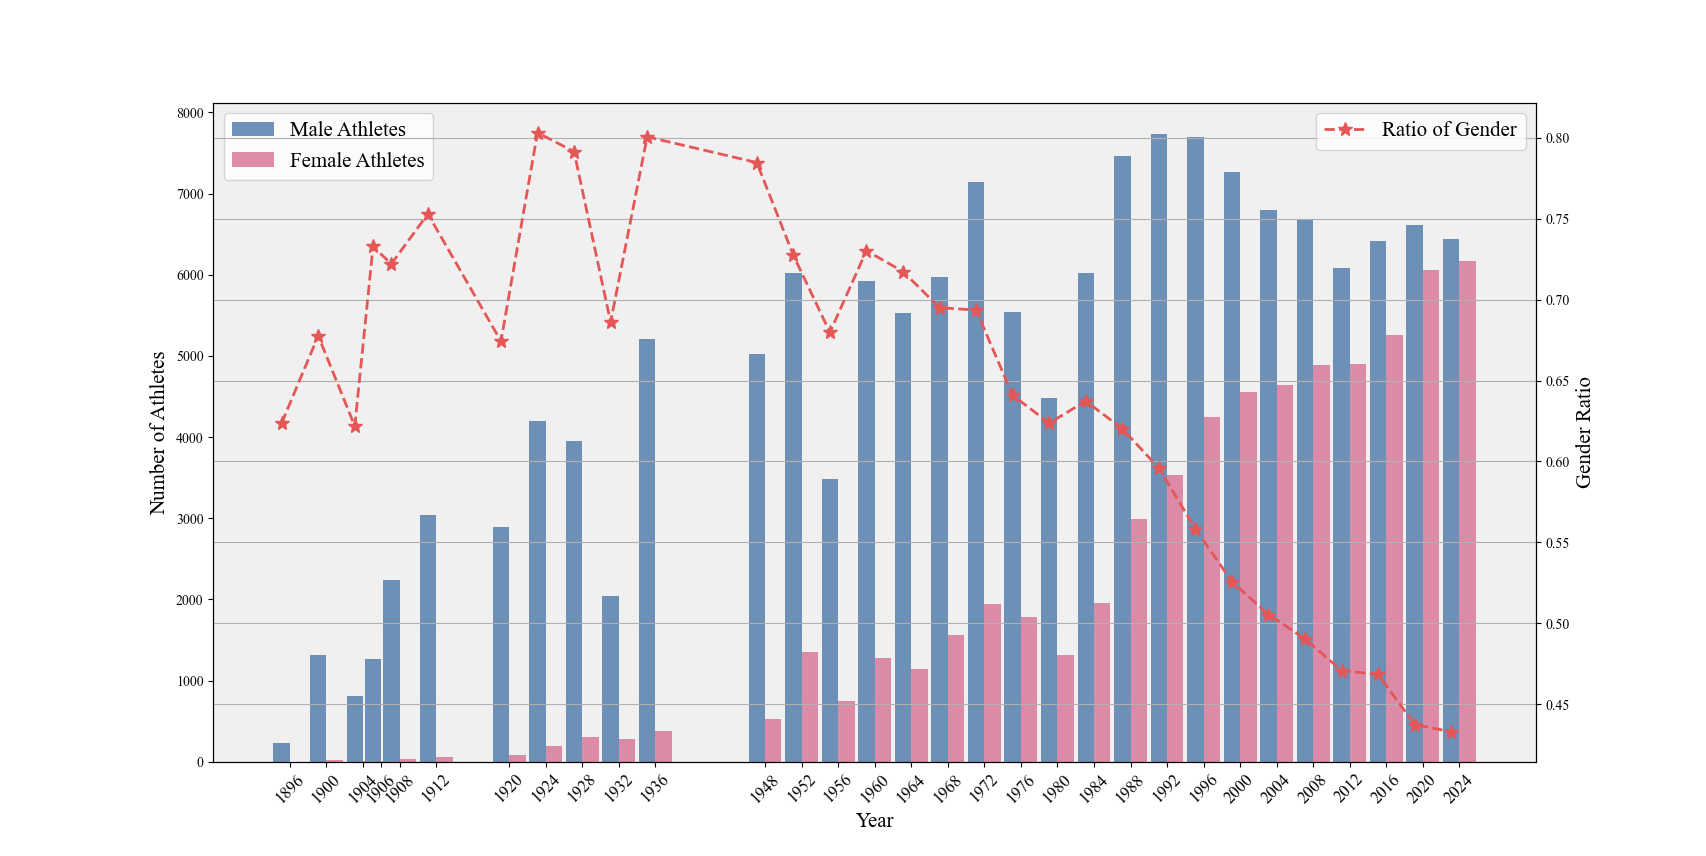
\includegraphics[width=16cm]{img/Gender with Award.png}
	\caption{Gender Distribution of Athletes(with Award)}
	\label{fig:aa}
\end{figure}

\begin{figure}[htbp]
	\centering
	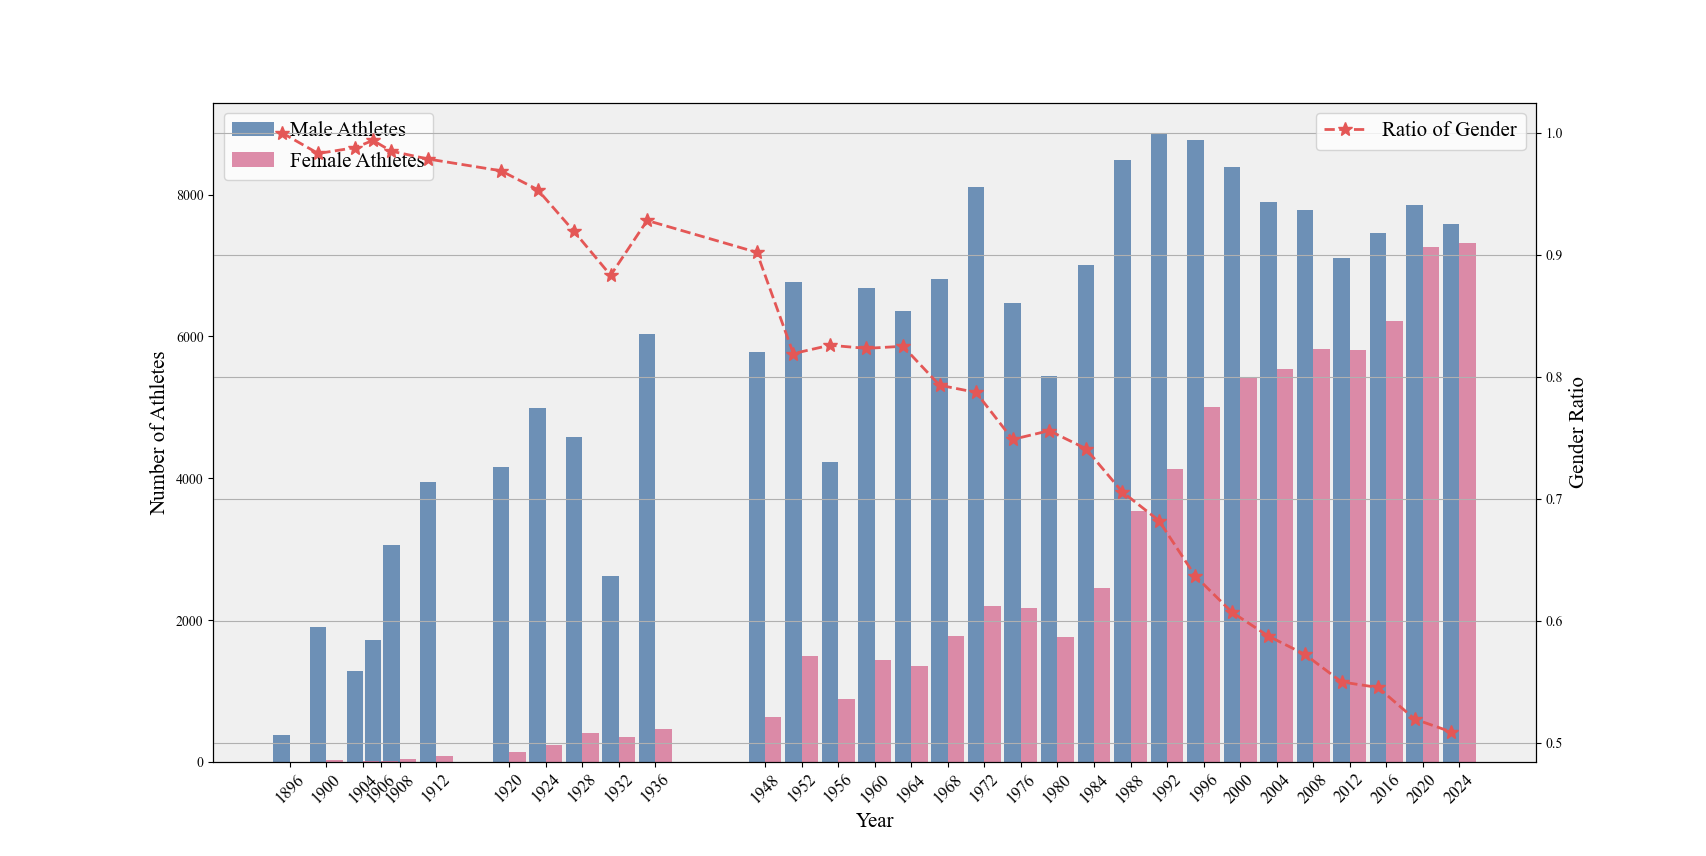
\includegraphics[width=16cm]{img/Gender.png}
	\caption{Gender Distribution of Athletes}
	\label{fig:aa}
\end{figure}

%6.2
\subsection{Strength events}


%6.3
\subsection{Global Geopolitics}


%6.3 花里胡哨图
\begin{figure}[htbp]
	\centering
	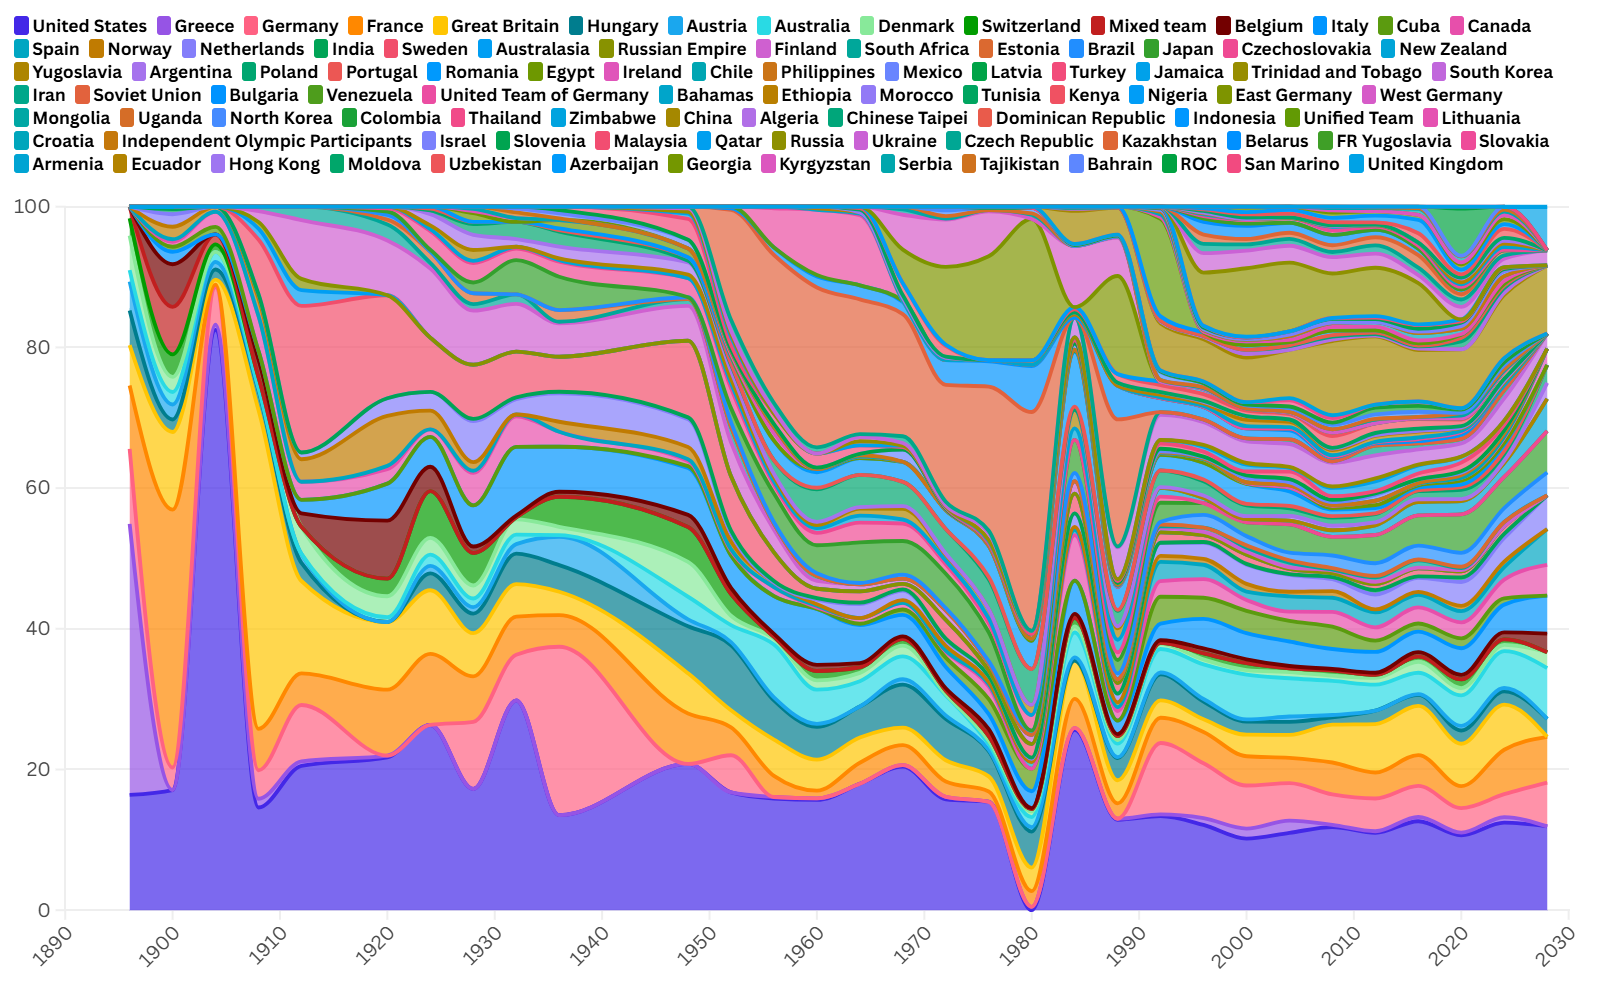
\includegraphics[width=16cm]{img/3.3-1.png}
	\caption{Trend of Medal Proportions by Country Annually}
	\label{fig:aa}
\end{figure}








\section{Sensitivity Analysis}

\begin{figure}[htbp]
	\centering
	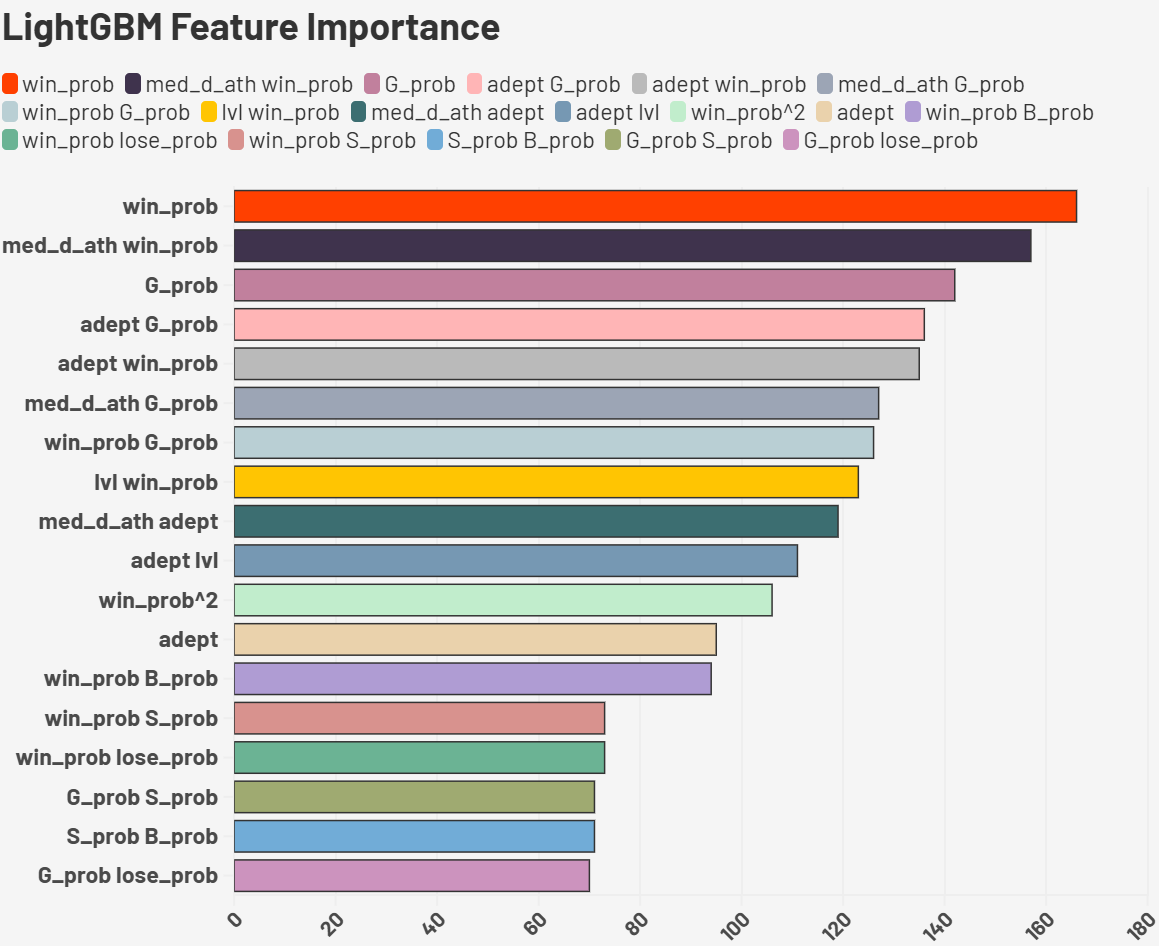
\includegraphics[width=16cm]{img/Sensitive Analysis 1.png}
	\caption{LightGBM Feature Importance}
	\label{fig:aa}
\end{figure}

\begin{figure}[htbp]
	\centering
	\begin{subfigure}[b]{.32\textwidth}
		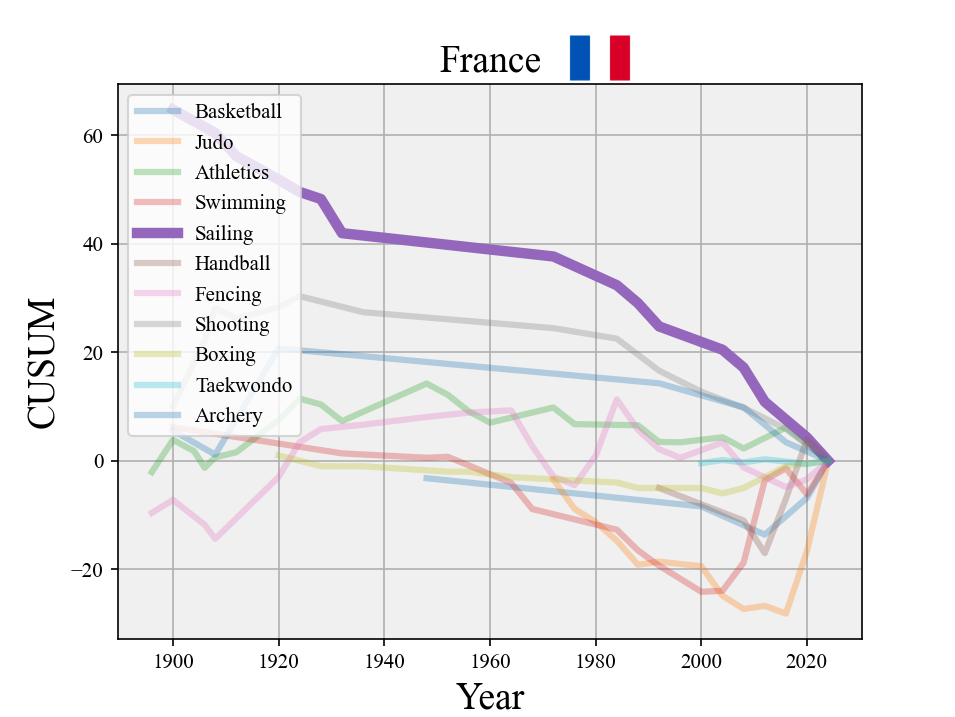
\includegraphics[width=\textwidth]{img/Decline1.png}
		\caption{France}\label{subfig:1}
	\end{subfigure}
	\hfill 
	\begin{subfigure}[b]{.32\textwidth}
		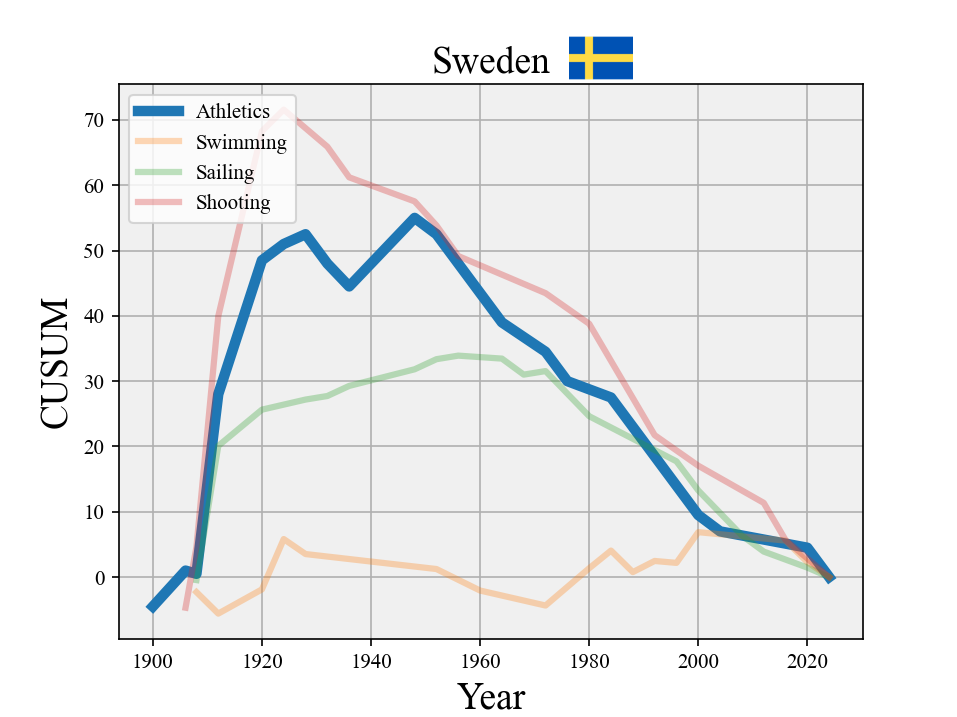
\includegraphics[width=\textwidth]{img/Decline2.png}
		\caption{Sweden}\label{subfig:2}
	\end{subfigure}
	\hfill 
	\begin{subfigure}[b]{.32\textwidth}
		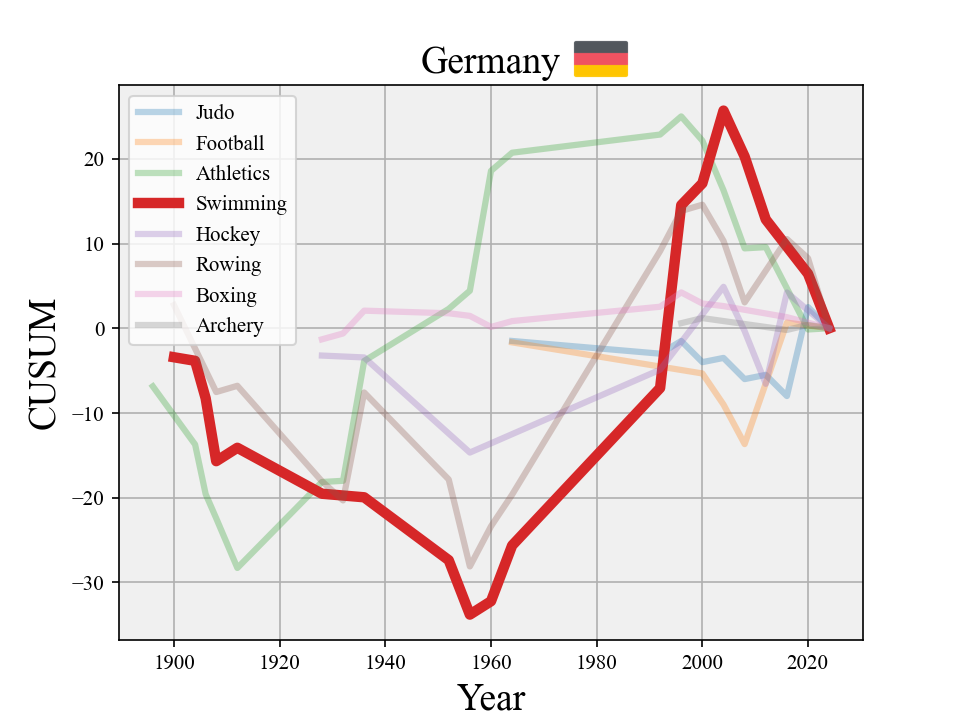
\includegraphics[width=\textwidth]{img/Decline3.png}
		\caption{Germany}\label{subfig:3}
	\end{subfigure}
	\caption{Three images}\label{fig:subfigures}
\end{figure}





\section{Model Evaluation}
\subsection{Strengths}
1.

2. 

3. 

4. 
\subsection{Weaknesses}
1.

 	
 	

\section{Conclusion}
\begin{itemize}
	\item Task1
	
	 \qquad AA\\
	bbb
	
	\item Task2\\
	\qquad AAA
	\item Task3\\
	\qquad AAA
	
	\item Task4\\
	\qquad AAA
	
\end{itemize}


% 参考文献,此处以 MLA 引用格式为例
\begin{thebibliography}{99}
\bibitem{1} Einstein, A., Podolsky, B., \& Rosen, N. (1935). Can quantum-mechanical description of physical reality be considered complete?. \emph{Physical review}, 47(10), 777.
\bibitem{2} \emph{A simple, easy \LaTeX\ template for MCM/ICM: EasyMCM}. (2018). Retrieved December 1, 2019, from\url{https://www.cnblogs.com/xjtu-blacksmith/p/easymcm.html}
\end{thebibliography}







% 以下为附录内容
% 如您的论文中不需要附录,请自行删除
\begin{subappendices}  % 附录环境


\section{Appendix A: Countries' Medal Count Prediction}

\begin{longtable}{|l|c|c|c|c|c|c|c|c|c|c|}
	\caption{Countries' Medal Count Prediction}\\
	\hline
	Country                                                        & \multicolumn{1}{l|}{\begin{tabular}[c]{@{}l@{}}G\_\\pes.\end{tabular}} & \multicolumn{1}{l|}{\begin{tabular}[c]{@{}l@{}}S\_\\pes.\end{tabular}} & \multicolumn{1}{l|}{\begin{tabular}[c]{@{}l@{}}B\_\\pes.\end{tabular}} & \multicolumn{1}{l|}{\begin{tabular}[c]{@{}l@{}}G\_\\opt.\end{tabular}} & \multicolumn{1}{l|}{\begin{tabular}[c]{@{}l@{}}S\_\\opt.\end{tabular}} & \multicolumn{1}{l|}{\begin{tabular}[c]{@{}l@{}}B\_\\opt.\end{tabular}} & \multicolumn{1}{l|}{Gold} & \multicolumn{1}{l|}{Silver} & \multicolumn{1}{l|}{Bronze} & \multicolumn{1}{l|}{Total}  \endfirsthead 
	\hline
	United States                                                  & 47                                                                     & 36                                                                     & 23                                                                     & 53                                                                     & 41                                                                     & 25                                                                     & 51                        & 40                          & 25                          & 117                         \\ 
	\hline
	China                                                          & 35                                                                     & 35                                                                     & 15                                                                     & 46                                                                     & 38                                                                     & 20                                                                     & 40                        & 36                          & 17                          & 95                          \\ 
	\hline
	Australia                                                      & 28                                                                     & 20                                                                     & 22                                                                     & 33                                                                     & 24                                                                     & 24                                                                     & 29                        & 22                          & 23                          & 71                          \\ 
	\hline
	France                                                         & 23                                                                     & 19                                                                     & 19                                                                     & 27                                                                     & 20                                                                     & 22                                                                     & 24                        & 19                          & 21                          & 64                          \\ 
	\hline
	Germany                                                        & 18                                                                     & 24                                                                     & 14                                                                     & 23                                                                     & 26                                                                     & 16                                                                     & 21                        & 25                          & 15                          & 61                          \\ 
	\hline
	United Kingdom                                                 & 20                                                                     & 19                                                                     & 14                                                                     & 26                                                                     & 24                                                                     & 15                                                                     & 25                        & 21                          & 15                          & 61                          \\ 
	\hline
	Japan                                                          & 16                                                                     & 25                                                                     & 14                                                                     & 19                                                                     & 27                                                                     & 16                                                                     & 17                        & 26                          & 16                          & 58                          \\ 
	\hline
	Italy                                                          & 15                                                                     & 20                                                                     & 15                                                                     & 17                                                                     & 20                                                                     & 22                                                                     & 16                        & 20                          & 16                          & 53                          \\ 
	\hline
	Spain                                                          & 21                                                                     & 10                                                                     & 13                                                                     & 30                                                                     & 12                                                                     & 14                                                                     & 25                        & 12                          & 13                          & 50                          \\ 
	\hline
	Netherlands                                                    & 24                                                                     & 6                                                                      & 13                                                                     & 29                                                                     & 9                                                                      & 15                                                                     & 26                        & 8                           & 15                          & 47                          \\ 
	\hline
	New Zealand                                                    & 20                                                                     & 13                                                                     & 9                                                                      & 22                                                                     & 15                                                                     & 10                                                                     & 22                        & 14                          & 9                           & 45                          \\ 
	\hline
	Canada                                                         & 15                                                                     & 10                                                                     & 16                                                                     & 19                                                                     & 10                                                                     & 18                                                                     & 17                        & 10                          & 16                          & 43                          \\ 
	\hline
	Brazil                                                         & 8                                                                      & 10                                                                     & 13                                                                     & 8                                                                      & 11                                                                     & 15                                                                     & 8                         & 10                          & 14                          & 32                          \\ 
	\hline
	Belgium                                                        & 6                                                                      & 8                                                                      & 7                                                                      & 15                                                                     & 10                                                                     & 8                                                                      & 11                        & 8                           & 7                           & 26                          \\ 
	\hline
	Hungary                                                        & 7                                                                      & 6                                                                      & 8                                                                      & 8                                                                      & 8                                                                      & 9                                                                      & 8                         & 8                           & 9                           & 25                          \\ 
	\hline
	Poland                                                         & 10                                                                     & 7                                                                      & 6                                                                      & 12                                                                     & 10                                                                     & 8                                                                      & 11                        & 9                           & 6                           & 25                          \\ 
	\hline
	Ireland                                                        & 6                                                                      & 10                                                                     & 6                                                                      & 7                                                                      & 11                                                                     & 6                                                                      & 6                         & 10                          & 6                           & 23                          \\ 
	\hline
	Argentina                                                      & 4                                                                      & 8                                                                      & 7                                                                      & 5                                                                      & 10                                                                     & 9                                                                      & 4                         & 9                           & 8                           & 22                          \\ 
	\hline
	Denmark                                                        & 10                                                                     & 7                                                                      & 5                                                                      & 12                                                                     & 8                                                                      & 8                                                                      & 10                        & 8                           & 6                           & 22                          \\ 
	\hline
	Ukraine                                                        & 3                                                                      & 7                                                                      & 8                                                                      & 5                                                                      & 8                                                                      & 9                                                                      & 4                         & 8                           & 8                           & 21                          \\ 
	\hline
	South Korea                                                    & 10                                                                     & 5                                                                      & 4                                                                      & 12                                                                     & 6                                                                      & 4                                                                      & 11                        & 6                           & 4                           & 21                          \\ 
	\hline
	Romania                                                        & 10                                                                     & 7                                                                      & 3                                                                      & 12                                                                     & 8                                                                      & 3                                                                      & 12                        & 7                           & 3                           & 20                          \\ 
	\hline
	Norway                                                         & 11                                                                     & 1                                                                      & 4                                                                      & 11                                                                     & 3                                                                      & 6                                                                      & 11                        & 2                           & 6                           & 19                          \\ 
	\hline
	South Africa                                                   & 6                                                                      & 4                                                                      & 4                                                                      & 8                                                                      & 8                                                                      & 5                                                                      & 8                         & 7                           & 5                           & 18                          \\ 
	\hline
	Slovenia                                                       & 4                                                                      & 3                                                                      & 8                                                                      & 6                                                                      & 3                                                                      & 8                                                                      & 4                         & 3                           & 8                           & 17                          \\ 
	\hline
	Kenya                                                          & 5                                                                      & 4                                                                      & 4                                                                      & 5                                                                      & 7                                                                      & 5                                                                      & 5                         & 7                           & 4                           & 16                          \\ 
	\hline
	Serbia                                                         & 4                                                                      & 5                                                                      & 6                                                                      & 5                                                                      & 9                                                                      & 7                                                                      & 4                         & 8                           & 6                           & 16                          \\ 
	\hline
	Mexico                                                         & 4                                                                      & 4                                                                      & 3                                                                      & 6                                                                      & 4                                                                      & 5                                                                      & 5                         & 4                           & 4                           & 15                          \\ 
	\hline
	India                                                          & 1                                                                      & 1                                                                      & 4                                                                      & 8                                                                      & 4                                                                      & 5                                                                      & 7                         & 3                           & 4                           & 15                          \\ 
	\hline
	Greece                                                         & 3                                                                      & 4                                                                      & 2                                                                      & 7                                                                      & 4                                                                      & 3                                                                      & 7                         & 4                           & 3                           & 14                          \\ 
	\hline
	Switzerland                                                    & 2                                                                      & 4                                                                      & 5                                                                      & 5                                                                      & 4                                                                      & 6                                                                      & 4                         & 4                           & 6                           & 14                          \\ 
	\hline
	Jamaica                                                        & 1                                                                      & 7                                                                      & 2                                                                      & 5                                                                      & 12                                                                     & 3                                                                      & 4                         & 8                           & 2                           & 13                          \\ 
	\hline
	Czech Republic                                                 & 5                                                                      & 3                                                                      & 3                                                                      & 6                                                                      & 4                                                                      & 5                                                                      & 6                         & 4                           & 4                           & 13                          \\ 
	\hline
	Uzbekistan                                                     & 4                                                                      & 2                                                                      & 2                                                                      & 5                                                                      & 3                                                                      & 2                                                                      & 4                         & 2                           & 2                           & 10                          \\ 
	\hline
	Nigeria                                                        & 4                                                                      & 2                                                                      & 4                                                                      & 4                                                                      & 3                                                                      & 4                                                                      & 4                         & 2                           & 4                           & 10                          \\ 
	\hline
	Sweden                                                         & 4                                                                      & 4                                                                      & 2                                                                      & 5                                                                      & 5                                                                      & 5                                                                      & 4                         & 4                           & 2                           & 10                          \\ 
	\hline
	Turkey                                                         & 3                                                                      & 2                                                                      & 5                                                                      & 3                                                                      & 2                                                                      & 6                                                                      & 3                         & 2                           & 5                           & 10                          \\ 
	\hline
	Finland                                                        & 2                                                                      & 6                                                                      & 2                                                                      & 2                                                                      & 6                                                                      & 2                                                                      & 2                         & 6                           & 2                           & 10                          \\ 
	\hline
	Colombia                                                       & 5                                                                      & 2                                                                      & 0                                                                      & 5                                                                      & 3                                                                      & 1                                                                      & 5                         & 3                           & 0                           & 9                           \\ 
	\hline
	Egypt                                                          & 0                                                                      & 3                                                                      & 3                                                                      & 1                                                                      & 4                                                                      & 4                                                                      & 0                         & 4                           & 4                           & 8                           \\ 
	\hline
	Kazakhstan                                                     & 1                                                                      & 2                                                                      & 2                                                                      & 4                                                                      & 4                                                                      & 2                                                                      & 3                         & 3                           & 2                           & 8                           \\ 
	\hline
	Iran                                                           & 2                                                                      & 2                                                                      & 1                                                                      & 5                                                                      & 3                                                                      & 2                                                                      & 4                         & 2                           & 1                           & 8                           \\ 
	\hline
	\begin{tabular}[c]{@{}l@{}}Dominican \\Republic\end{tabular}   & 3                                                                      & 3                                                                      & 2                                                                      & 6                                                                      & 4                                                                      & 3                                                                      & 5                         & 3                           & 3                           & 8                           \\ 
	\hline
	Portugal                                                       & 2                                                                      & 3                                                                      & 3                                                                      & 2                                                                      & 4                                                                      & 3                                                                      & 2                         & 3                           & 3                           & 8                           \\ 
	\hline
	Cuba                                                           & 2                                                                      & 2                                                                      & 1                                                                      & 3                                                                      & 2                                                                      & 2                                                                      & 3                         & 2                           & 2                           & 7                           \\ 
	\hline
	Unknown                                                        & 1                                                                      & 2                                                                      & 2                                                                      & 1                                                                      & 2                                                                      & 4                                                                      & 1                         & 2                           & 2                           & 7                           \\ 
	\hline
	Latvia                                                         & 3                                                                      & 1                                                                      & 3                                                                      & 3                                                                      & 1                                                                      & 3                                                                      & 3                         & 1                           & 3                           & 7                           \\ 
	\hline
	Ethiopia                                                       & 2                                                                      & 1                                                                      & 0                                                                      & 2                                                                      & 6                                                                      & 2                                                                      & 2                         & 2                           & 2                           & 6                           \\ 
	\hline
	Algeria                                                        & 2                                                                      & 2                                                                      & 1                                                                      & 2                                                                      & 3                                                                      & 2                                                                      & 2                         & 2                           & 1                           & 6                           \\ 
	\hline
	Morocco                                                        & 0                                                                      & 2                                                                      & 4                                                                      & 0                                                                      & 2                                                                      & 5                                                                      & 0                         & 2                           & 5                           & 6                           \\ 
	\hline
	Austria                                                        & 3                                                                      & 0                                                                      & 1                                                                      & 3                                                                      & 1                                                                      & 2                                                                      & 3                         & 0                           & 2                           & 6                           \\ 
	\hline
	Puerto Rico                                                    & 2                                                                      & 3                                                                      & 1                                                                      & 4                                                                      & 3                                                                      & 2                                                                      & 2                         & 3                           & 2                           & 6                           \\ 
	\hline
	Thailand                                                       & 1                                                                      & 2                                                                      & 1                                                                      & 2                                                                      & 2                                                                      & 2                                                                      & 2                         & 2                           & 1                           & 5                           \\ 
	\hline
	Croatia                                                        & 2                                                                      & 2                                                                      & 0                                                                      & 2                                                                      & 2                                                                      & 1                                                                      & 2                         & 2                           & 1                           & 5                           \\ 
	\hline
	Ecuador                                                        & 2                                                                      & 0                                                                      & 2                                                                      & 3                                                                      & 1                                                                      & 3                                                                      & 2                         & 0                           & 3                           & 5                           \\ 
	\hline
	Uganda                                                         & 0                                                                      & 1                                                                      & 1                                                                      & 1                                                                      & 4                                                                      & 1                                                                      & 1                         & 3                           & 1                           & 5                           \\ 
	\hline
	Angola                                                         & 0                                                                      & 2                                                                      & 0                                                                      & 1                                                                      & 3                                                                      & 1                                                                      & 0                         & 2                           & 0                           & 5                           \\ 
	\hline
	Israel                                                         & 2                                                                      & 2                                                                      & 1                                                                      & 2                                                                      & 2                                                                      & 2                                                                      & 2                         & 2                           & 1                           & 5                           \\ 
	\hline
	Mongolia                                                       & 1                                                                      & 3                                                                      & 1                                                                      & 1                                                                      & 4                                                                      & 1                                                                      & 1                         & 4                           & 1                           & 5                           \\ 
	\hline
	Fiji                                                           & 0                                                                      & 1                                                                      & 0                                                                      & 2                                                                      & 5                                                                      & 1                                                                      & 1                         & 4                           & 0                           & 5                           \\ 
	\hline
	Uruguay                                                        & 0                                                                      & 2                                                                      & 0                                                                      & 1                                                                      & 3                                                                      & 1                                                                      & 0                         & 2                           & 0                           & 5                           \\ 
	\hline
	Chile                                                          & 0                                                                      & 2                                                                      & 0                                                                      & 1                                                                      & 3                                                                      & 1                                                                      & 0                         & 2                           & 0                           & 5                           \\ 
	\hline
	Unknown                                                        & 1                                                                      & 1                                                                      & 0                                                                      & 3                                                                      & 1                                                                      & 0                                                                      & 1                         & 1                           & 0                           & 4                           \\ 
	\hline
	Zambia                                                         & 1                                                                      & 3                                                                      & 0                                                                      & 1                                                                      & 3                                                                      & 0                                                                      & 1                         & 3                           & 0                           & 4                           \\ 
	\hline
	Azerbaijan                                                     & 1                                                                      & 0                                                                      & 2                                                                      & 1                                                                      & 1                                                                      & 2                                                                      & 1                         & 1                           & 2                           & 4                           \\ 
	\hline
	Guinea                                                         & 0                                                                      & 4                                                                      & 0                                                                      & 0                                                                      & 4                                                                      & 0                                                                      & 0                         & 4                           & 0                           & 4                           \\ 
	\hline
	Georgia                                                        & 1                                                                      & 1                                                                      & 0                                                                      & 2                                                                      & 2                                                                      & 0                                                                      & 2                         & 2                           & 0                           & 3                           \\ 
	\hline
	Mali                                                           & 0                                                                      & 3                                                                      & 0                                                                      & 0                                                                      & 3                                                                      & 0                                                                      & 0                         & 3                           & 0                           & 3                           \\ 
	\hline
	\begin{tabular}[c]{@{}l@{}}Chinese\\Taipei\end{tabular}        & 2                                                                      & 1                                                                      & 0                                                                      & 2                                                                      & 1                                                                      & 0                                                                      & 2                         & 1                           & 0                           & 3                           \\ 
	\hline
	Venezuela                                                      & 0                                                                      & 2                                                                      & 1                                                                      & 1                                                                      & 2                                                                      & 2                                                                      & 0                         & 2                           & 2                           & 3                           \\ 
	\hline
	Paraguay                                                       & 0                                                                      & 3                                                                      & 0                                                                      & 0                                                                      & 4                                                                      & 0                                                                      & 0                         & 4                           & 0                           & 3                           \\ 
	\hline
	Indonesia                                                      & 0                                                                      & 1                                                                      & 1                                                                      & 1                                                                      & 1                                                                      & 2                                                                      & 1                         & 1                           & 2                           & 3                           \\ 
	\hline
	Peru                                                           & 0                                                                      & 1                                                                      & 0                                                                      & 1                                                                      & 2                                                                      & 0                                                                      & 0                         & 2                           & 0                           & 3                           \\ 
	\hline
	Iraq                                                           & 0                                                                      & 3                                                                      & 0                                                                      & 0                                                                      & 3                                                                      & 0                                                                      & 0                         & 3                           & 0                           & 3                           \\ 
	\hline
	Bulgaria                                                       & 1                                                                      & 1                                                                      & 0                                                                      & 1                                                                      & 1                                                                      & 1                                                                      & 1                         & 1                           & 0                           & 3                           \\ 
	\hline
	Lithuania                                                      & 2                                                                      & 1                                                                      & 0                                                                      & 2                                                                      & 2                                                                      & 1                                                                      & 2                         & 1                           & 1                           & 3                           \\ 
	\hline
	Tunisia                                                        & 0                                                                      & 0                                                                      & 0                                                                      & 1                                                                      & 1                                                                      & 0                                                                      & 0                         & 0                           & 0                           & 2                           \\ 
	\hline
	Guatemala                                                      & 1                                                                      & 0                                                                      & 1                                                                      & 1                                                                      & 0                                                                      & 1                                                                      & 1                         & 0                           & 1                           & 2                           \\ 
	\hline
	Bahamas                                                        & 0                                                                      & 2                                                                      & 0                                                                      & 1                                                                      & 2                                                                      & 0                                                                      & 0                         & 2                           & 0                           & 2                           \\ 
	\hline
	\begin{tabular}[c]{@{}l@{}}Trinidad and \\Tobago\end{tabular}  & 0                                                                      & 1                                                                      & 0                                                                      & 1                                                                      & 1                                                                      & 0                                                                      & 0                         & 1                           & 0                           & 2                           \\ 
	\hline
	Montenegro                                                     & 0                                                                      & 1                                                                      & 0                                                                      & 0                                                                      & 2                                                                      & 0                                                                      & 0                         & 2                           & 0                           & 2                           \\ 
	\hline
	Hong Kong                                                      & 0                                                                      & 1                                                                      & 1                                                                      & 0                                                                      & 1                                                                      & 1                                                                      & 0                         & 1                           & 1                           & 2                           \\ 
	\hline
	Moldova                                                        & 0                                                                      & 1                                                                      & 0                                                                      & 0                                                                      & 2                                                                      & 0                                                                      & 0                         & 2                           & 0                           & 1                           \\ 
	\hline
	South Sudan                                                    & 0                                                                      & 1                                                                      & 0                                                                      & 0                                                                      & 2                                                                      & 0                                                                      & 0                         & 2                           & 0                           & 1                           \\ 
	\hline
	Malaysia                                                       & 0                                                                      & 1                                                                      & 0                                                                      & 0                                                                      & 1                                                                      & 0                                                                      & 0                         & 1                           & 0                           & 1                           \\ 
	\hline
	Philippines                                                    & 0                                                                      & 0                                                                      & 0                                                                      & 1                                                                      & 0                                                                      & 0                                                                      & 0                         & 0                           & 0                           & 1                           \\ 
	\hline
	Bahrain                                                        & 0                                                                      & 0                                                                      & 0                                                                      & 0                                                                      & 2                                                                      & 0                                                                      & 0                         & 1                           & 0                           & 1                           \\ 
	\hline
	Estonia                                                        & 0                                                                      & 0                                                                      & 1                                                                      & 0                                                                      & 0                                                                      & 1                                                                      & 0                         & 0                           & 1                           & 1                           \\ 
	\hline
	Liberia                                                        & 0                                                                      & 1                                                                      & 0                                                                      & 0                                                                      & 2                                                                      & 0                                                                      & 0                         & 1                           & 0                           & 1                           \\ 
	\hline
	\begin{tabular}[c]{@{}l@{}}United Arab \\Emirates\end{tabular} & 0                                                                      & 0                                                                      & 0                                                                      & 0                                                                      & 1                                                                      & 0                                                                      & 0                         & 0                           & 0                           & 1                           \\ 
	\hline
	Jordan                                                         & 0                                                                      & 0                                                                      & 0                                                                      & 0                                                                      & 1                                                                      & 0                                                                      & 0                         & 0                           & 0                           & 1                           \\ 
	\hline
	Eritrea                                                        & 0                                                                      & 1                                                                      & 0                                                                      & 0                                                                      & 2                                                                      & 0                                                                      & 0                         & 2                           & 0                           & 1                           \\ 
	\hline
	Singapore                                                      & 0                                                                      & 0                                                                      & 0                                                                      & 0                                                                      & 1                                                                      & 1                                                                      & 0                         & 0                           & 1                           & 1                           \\ 
	\hline
	Luxembourg                                                     & 0                                                                      & 0                                                                      & 0                                                                      & 0                                                                      & 1                                                                      & 0                                                                      & 0                         & 0                           & 0                           & 1                           \\ 
	\hline
	Cyprus                                                         & 0                                                                      & 0                                                                      & 0                                                                      & 0                                                                      & 1                                                                      & 0                                                                      & 0                         & 0                           & 0                           & 1                           \\ 
	\hline
	Samoa                                                          & 0                                                                      & 1                                                                      & 0                                                                      & 0                                                                      & 1                                                                      & 0                                                                      & 0                         & 1                           & 0                           & 1                           \\ 
	\hline
	Qatar                                                          & 0                                                                      & 0                                                                      & 0                                                                      & 0                                                                      & 0                                                                      & 0                                                                      & 0                         & 0                           & 0                           & 0                           \\ 
	\hline
	Tanzania                                                       & 0                                                                      & 0                                                                      & 0                                                                      & 0                                                                      & 0                                                                      & 0                                                                      & 0                         & 0                           & 0                           & 0                           \\ 
	\hline
	Djibouti                                                       & 0                                                                      & 0                                                                      & 0                                                                      & 0                                                                      & 0                                                                      & 0                                                                      & 0                         & 0                           & 0                           & 0                           \\ 
	\hline
	Ghana                                                          & 0                                                                      & 0                                                                      & 0                                                                      & 0                                                                      & 0                                                                      & 0                                                                      & 0                         & 0                           & 0                           & 0                           \\ 
	\hline
	Ivory Coast                                                    & 0                                                                      & 0                                                                      & 0                                                                      & 0                                                                      & 0                                                                      & 0                                                                      & 0                         & 0                           & 0                           & 0                           \\ 
	\hline
	Tajikistan                                                     & 0                                                                      & 0                                                                      & 0                                                                      & 0                                                                      & 0                                                                      & 0                                                                      & 0                         & 0                           & 0                           & 0                           \\ 
	\hline
	Kyrgyzstan                                                     & 0                                                                      & 0                                                                      & 0                                                                      & 0                                                                      & 1                                                                      & 0                                                                      & 0                         & 0                           & 0                           & 0                           \\ 
	\hline
	Armenia                                                        & 0                                                                      & 0                                                                      & 0                                                                      & 0                                                                      & 0                                                                      & 0                                                                      & 0                         & 0                           & 0                           & 0                           \\ 
	\hline
	Slovakia                                                       & 0                                                                      & 0                                                                      & 0                                                                      & 0                                                                      & 0                                                                      & 0                                                                      & 0                         & 0                           & 0                           & 0                           \\ 
	\hline
	Botswana                                                       & 0                                                                      & 0                                                                      & 0                                                                      & 0                                                                      & 2                                                                      & 0                                                                      & 0                         & 0                           & 0                           & 0                           \\ 
	\hline
	Grenada                                                        & 0                                                                      & 0                                                                      & 0                                                                      & 0                                                                      & 0                                                                      & 0                                                                      & 0                         & 0                           & 0                           & 0                           \\ 
	\hline
	Zimbabwe                                                       & 0                                                                      & 0                                                                      & 0                                                                      & 0                                                                      & 0                                                                      & 0                                                                      & 0                         & 0                           & 0                           & 0                           \\ 
	\hline
	Burundi                                                        & 0                                                                      & 0                                                                      & 0                                                                      & 0                                                                      & 0                                                                      & 0                                                                      & 0                         & 0                           & 0                           & 0                           \\ 
	\hline
	Kosovo                                                         & 0                                                                      & 0                                                                      & 0                                                                      & 0                                                                      & 0                                                                      & 0                                                                      & 0                         & 0                           & 0                           & 0                           \\
	\hline
\end{longtable}



\section{Appendix B: Program Codes}
Here are the program codes we used in our research.

% 代码环境示例三则
% 如您的论文不需要展示代码,请删除
% 更多用法,请参考 listings 宏包文档

% Python 代码示例
\begin{lstlisting}[language=Python, name={test.py}]
# Python code example
for i in range(10):
    print('Hello, world!')
\end{lstlisting}

% MATLAB 代码示例
\begin{lstlisting}[language=MATLAB, name={test.m}]
% MATLAB code example
for i = 1:10
    disp("hello, world!");
end
\end{lstlisting}



% C++ 代码示例
\begin{lstlisting}[language=C++, name={test.cpp}]
// C++ code example
#include <iostream>
using namespace std;

int main() {
    for (int i = 0; i < 10; i++)
        cout << "hello, world" << endl;
    return 0;
}
\end{lstlisting}

\end{subappendices}  % 附录内容结束

\end{document}  % 结束
